% Options for packages loaded elsewhere
\PassOptionsToPackage{unicode}{hyperref}
\PassOptionsToPackage{hyphens}{url}
%
\documentclass[
  english,
  man,floatsintext]{apa6}
\usepackage{amsmath,amssymb}
\usepackage{lmodern}
\usepackage{ifxetex,ifluatex}
\ifnum 0\ifxetex 1\fi\ifluatex 1\fi=0 % if pdftex
  \usepackage[T1]{fontenc}
  \usepackage[utf8]{inputenc}
  \usepackage{textcomp} % provide euro and other symbols
\else % if luatex or xetex
  \usepackage{unicode-math}
  \defaultfontfeatures{Scale=MatchLowercase}
  \defaultfontfeatures[\rmfamily]{Ligatures=TeX,Scale=1}
\fi
% Use upquote if available, for straight quotes in verbatim environments
\IfFileExists{upquote.sty}{\usepackage{upquote}}{}
\IfFileExists{microtype.sty}{% use microtype if available
  \usepackage[]{microtype}
  \UseMicrotypeSet[protrusion]{basicmath} % disable protrusion for tt fonts
}{}
\makeatletter
\@ifundefined{KOMAClassName}{% if non-KOMA class
  \IfFileExists{parskip.sty}{%
    \usepackage{parskip}
  }{% else
    \setlength{\parindent}{0pt}
    \setlength{\parskip}{6pt plus 2pt minus 1pt}}
}{% if KOMA class
  \KOMAoptions{parskip=half}}
\makeatother
\usepackage{xcolor}
\IfFileExists{xurl.sty}{\usepackage{xurl}}{} % add URL line breaks if available
\IfFileExists{bookmark.sty}{\usepackage{bookmark}}{\usepackage{hyperref}}
\hypersetup{
  pdftitle={Cognitive Music Listening Space: A Multivariate Approach},
  pdfauthor={Brendon Mizener1, Mathilde Vandenberghe2, Hervé Abdi1, \& Sylvie Chollet2},
  pdflang={en-EN},
  pdfkeywords={Music, Perception, Cognition, Multivariate Analyses},
  hidelinks,
  pdfcreator={LaTeX via pandoc}}
\urlstyle{same} % disable monospaced font for URLs
\usepackage{graphicx}
\makeatletter
\def\maxwidth{\ifdim\Gin@nat@width>\linewidth\linewidth\else\Gin@nat@width\fi}
\def\maxheight{\ifdim\Gin@nat@height>\textheight\textheight\else\Gin@nat@height\fi}
\makeatother
% Scale images if necessary, so that they will not overflow the page
% margins by default, and it is still possible to overwrite the defaults
% using explicit options in \includegraphics[width, height, ...]{}
\setkeys{Gin}{width=\maxwidth,height=\maxheight,keepaspectratio}
% Set default figure placement to htbp
\makeatletter
\def\fps@figure{htbp}
\makeatother
\setlength{\emergencystretch}{3em} % prevent overfull lines
\providecommand{\tightlist}{%
  \setlength{\itemsep}{0pt}\setlength{\parskip}{0pt}}
\setcounter{secnumdepth}{-\maxdimen} % remove section numbering
% Make \paragraph and \subparagraph free-standing
\ifx\paragraph\undefined\else
  \let\oldparagraph\paragraph
  \renewcommand{\paragraph}[1]{\oldparagraph{#1}\mbox{}}
\fi
\ifx\subparagraph\undefined\else
  \let\oldsubparagraph\subparagraph
  \renewcommand{\subparagraph}[1]{\oldsubparagraph{#1}\mbox{}}
\fi
% Manuscript styling
\usepackage{upgreek}
\captionsetup{font=singlespacing,justification=justified}

% Table formatting
\usepackage{longtable}
\usepackage{lscape}
% \usepackage[counterclockwise]{rotating}   % Landscape page setup for large tables
\usepackage{multirow}		% Table styling
\usepackage{tabularx}		% Control Column width
\usepackage[flushleft]{threeparttable}	% Allows for three part tables with a specified notes section
\usepackage{threeparttablex}            % Lets threeparttable work with longtable

% Create new environments so endfloat can handle them
% \newenvironment{ltable}
%   {\begin{landscape}\begin{center}\begin{threeparttable}}
%   {\end{threeparttable}\end{center}\end{landscape}}
\newenvironment{lltable}{\begin{landscape}\begin{center}\begin{ThreePartTable}}{\end{ThreePartTable}\end{center}\end{landscape}}

% Enables adjusting longtable caption width to table width
% Solution found at http://golatex.de/longtable-mit-caption-so-breit-wie-die-tabelle-t15767.html
\makeatletter
\newcommand\LastLTentrywidth{1em}
\newlength\longtablewidth
\setlength{\longtablewidth}{1in}
\newcommand{\getlongtablewidth}{\begingroup \ifcsname LT@\roman{LT@tables}\endcsname \global\longtablewidth=0pt \renewcommand{\LT@entry}[2]{\global\advance\longtablewidth by ##2\relax\gdef\LastLTentrywidth{##2}}\@nameuse{LT@\roman{LT@tables}} \fi \endgroup}

% \setlength{\parindent}{0.5in}
% \setlength{\parskip}{0pt plus 0pt minus 0pt}

% \usepackage{etoolbox}
\makeatletter
\patchcmd{\HyOrg@maketitle}
  {\section{\normalfont\normalsize\abstractname}}
  {\section*{\normalfont\normalsize\abstractname}}
  {}{\typeout{Failed to patch abstract.}}
\patchcmd{\HyOrg@maketitle}
  {\section{\protect\normalfont{\@title}}}
  {\section*{\protect\normalfont{\@title}}}
  {}{\typeout{Failed to patch title.}}
\makeatother
\shorttitle{Music Descriptor Space}
\keywords{Music, Perception, Cognition, Multivariate Analyses\newline\indent Word count: 5631}
\usepackage{csquotes}
\usepackage{caption}
\usepackage{subcaption}
\usepackage{wrapfig}
\ifxetex
  % Load polyglossia as late as possible: uses bidi with RTL langages (e.g. Hebrew, Arabic)
  \usepackage{polyglossia}
  \setmainlanguage[]{english}
\else
  \usepackage[main=english]{babel}
% get rid of language-specific shorthands (see #6817):
\let\LanguageShortHands\languageshorthands
\def\languageshorthands#1{}
\fi
\ifluatex
  \usepackage{selnolig}  % disable illegal ligatures
\fi
\newlength{\cslhangindent}
\setlength{\cslhangindent}{1.5em}
\newlength{\csllabelwidth}
\setlength{\csllabelwidth}{3em}
\newenvironment{CSLReferences}[2] % #1 hanging-ident, #2 entry spacing
 {% don't indent paragraphs
  \setlength{\parindent}{0pt}
  % turn on hanging indent if param 1 is 1
  \ifodd #1 \everypar{\setlength{\hangindent}{\cslhangindent}}\ignorespaces\fi
  % set entry spacing
  \ifnum #2 > 0
  \setlength{\parskip}{#2\baselineskip}
  \fi
 }%
 {}
\usepackage{calc}
\newcommand{\CSLBlock}[1]{#1\hfill\break}
\newcommand{\CSLLeftMargin}[1]{\parbox[t]{\csllabelwidth}{#1}}
\newcommand{\CSLRightInline}[1]{\parbox[t]{\linewidth - \csllabelwidth}{#1}\break}
\newcommand{\CSLIndent}[1]{\hspace{\cslhangindent}#1}

\title{Cognitive Music Listening Space: A Multivariate Approach}
\author{Brendon Mizener\textsuperscript{1}, Mathilde Vandenberghe\textsuperscript{2}, Hervé Abdi\textsuperscript{1}, \& Sylvie Chollet\textsuperscript{2}}
\date{}


\authornote{

Add complete departmental affiliations for each author here. Each new line herein must be indented, like this line.

Enter author note here.

The authors made the following contributions. Brendon Mizener: Stimuli creation, Survey design \& creation, Data collection \& processing, Statistical analyses, Writing - Original draft preparation; Mathilde Vandenberghe: Original concept, Survey design \& creation; Hervé Abdi: Writing - Review \& Editing, Statistical guidance; Sylvie Chollet: Original concept.

Correspondence concerning this article should be addressed to Brendon Mizener, 800 W. Campbell Rd., Richardson Tex. E-mail: \href{mailto:bmizener@utdallas.edu}{\nolinkurl{bmizener@utdallas.edu}}

}

\affiliation{\vspace{0.5cm}\textsuperscript{1} University of Texas at Dallas\\\textsuperscript{2} Junia, Univ. Artois, Université de Liège, Univ. Littoral Côte d'Opale, UMRT 1158 BioEcoAgro, F-62000 Arras, France}

\abstract{
French and American participants listened to new music stimuli and evaluated the stimuli using either adjectives or quantitative musical dimensions. Results were analyzed using Correspondence Analysis (CA), Hierarchical Cluster Analysis (HCA), Multiple Factor Analysis (MFA), and Partial Least Squares Correlation (PLSC). All except the HCA used Bootstrapping and Permutation testing for inferences. French and American listeners differed when they described the musical stimuli using adjectives, but not when using the quantitative dimensions. The present work serves as a case study in research methodology that allows for a balance between relaxing experimental control and maintaining statistical rigor.
}



\begin{document}
\maketitle

\begin{center}\rule{0.5\linewidth}{0.5pt}\end{center}

We have a data collection problem: World events over the last year have shown that we need to be able to collect good data outside of the lab. In the lab, because we control error sources, we measure, on relatively small sets of observations, a few well-defined, quantitative variables, analyzed using standard techniques such as analysis of variance (ANOVA). But, with the labs closed (remember COVID?), how can we collect good data? Away from the controlled environment of the lab, quantitative variables are hard to measure, but we can collect, on large sets of observations, qualitative variables that can only be analyzed by newer multivariate techniques. In the present paper, we present a case study illustrating this tradeoff.

``Doesn't beer taste better in a bar? Or when you're listening to your favorite song?'' The present study was designed to quantify a music listening `space' that captures objective stimulus and cognitive dimensions for the sake of investigating cross-modal sensory mapping between beer drinking and music listening. It also addresses other questions: Are there differences in how people from different countries --- and by extension musical cultures --- perceive and describe music? What parallels exist between stimulus dimensions and cognitive dimensions of music?

For the present study, we have defined stimulus dimensions as quantitative musical qualities, such as tempo, range, and meter and cognitive dimensions as qualitative descriptions of music, such as ``dark,'' ``warm,'' and ``round.'' These cognitive/qualitative dimensions are similar to the commonly investigated affective or emotional dimensions, but do not specifically assess affective quality. We designed three experiments to quantify individual and combined spaces for these concepts, using separate surveys. The first experiment included highly trained musicians and featured a multiple choice survey about the stimulus dimensions; the second included participants with any level of music training performing a check-all-that-apply task (CATA, Katz \& Braly, 1933; Meyners \& Castura, 2014; Coombs et al., 1956); the third experiment incorporated both surveys in a single analysis.

To analyze our data, we selected a set of multivariate analyses that allowed us to visualize answers to each of our questions. The mental spaces revealed by the individual surveys were calculated and visualized using Correspondence Analysis (CA), a method similar to Principal Components Analysis (PCA) that analyzes qualitative data. We used Multidimensional Scaling (MDS), a distance analysis, to visualize the differences between participants and participant groups. To find parallels between the surveys, we used Partial Least Squares Correlation (PLSC), a method that analyzes two data tables with different sets of variables measured on the same observations. We used a Multiple Factor Analysis to evaluate how French and American participants' responses differed. Each of these analyses provide different visualizations and interpretations of the data, which are discussed in more detail below.

\hypertarget{music-perception}{%
\subsection{Music Perception}\label{music-perception}}

Quantifying music perception is an interesting test case for this kind of data gathering and analytical paradigm. Most music or auditory perception studies have the inherent confound that small changes can affect listeners' perception, especially when the study involves timing, tuning, or sound localization. However, the experimental controls may be loosened slightly when investigating holistic music listening, because no single musical element is more important than the whole.

Quantitative and qualitative elements of music are theoretically distinct but practically inseparable (Bruner II, 1990). Listeners respond affectively to technical aspects of music using schemata informed by their individual musical experiences and personality traits (Kopacz, 2005), and composers use various musical and compositional techniques to convey the emotions they want to express (Battcock \& Schutz, 2019; Bruner II, 1990). However, quantifying the perceptual interactions between more than one or two musical qualities is a challenge. One reason is that models like ANOVA and its variations are limited by how many variables a researcher can include while remaining coherent. Another is that asking participants to respond to multiple aspects of a stimulus taxes participants' perceptual capacity and is thus difficult to measure (W. F. Thompson, 1994).

One specific area that has attempted to capture a greater dimensionality is music emotion research. This is a well trod domain --- see, for example Juslin and Sloboda (2010) --- and the application of multivariate analyses to these questions is similarly well established. Early studies, including Gray and Wheeler (1967), Wedin (1969), and Wedin (1972) used MDS to capture the affective space of various musical stimuli. MDS continues to be used commonly in more modern studies (Bigand et al., 2005; Madsen, 1997; Rodà et al., 2014), with a narrow focus on valence and arousal, which were first proposed to be the most salient dimensions of perception by Osgood and Suci (1955).

A few studies have specifically investigated dimensions beyond those first two (for example Rodà et al., 2014), and there are conflicting hypotheses about whether the valence-arousal plane a different model of emotion perception represents the fundamental space around music emotion perception (Cowen et al., 2020; Juslin \& Västfjäll, 2008). However, an important distinction between the present study and work in music emotion perception is that the adjectives we chose were informed by music composition and performance, rather than emotion (Wallmark, 2019).

With regard to trained and untrained musicians, there are many studies that evaluate their differences, but the verdict as to whether trained musicians are better music listeners is still out, partially due to the fact that there is little standardization in how much training is required for a participant to be ``highly trained'' (Bigand \& Poulin-Charronnat, 2006). There are, however, reported benefits with regard to sensitivity to the emotional content in music (Ladinig \& Glenn Schellenberg, 2012) and familiarity with tonal systems (Bartlett \& Dowling, 1980; Dowling, 1978). Recent works suggest that these benefits may be limited to specific technical aspects, and depend on the extent of training (Raman \& Dowling 2017). We included highly trained musicians because they are sensitive to these technical aspects of music and will be able to accurately quantify the stimuli. Additionally, some of the response options to questions on the survey for Experiment 1 would only be familiar to participants with significant music training.

\hypertarget{intercultural-music-perception}{%
\subsubsection{Intercultural music perception}\label{intercultural-music-perception}}

There are a few common goals in intercultural studies of music perception. Some quantify the shared emotional experience between musical cultures (L. L. Balkwill et al., 2004; L. Balkwill \& Thompson, 1999; Cowen et al., 2020; Darrow et al., 1987; Fritz et al., 2009; Gregory \& Varney, 1996), and some ask participants to identify technical aspects of music from other cultures (Raman \& Dowling, 2016, 2017). There are fewer studies that include semantics in their evaluation of music perception (Zacharakis et al., 2014, 2015), which makes this a prime area for research.

The research program presented in Zacharakis et al. (2014) and Zacharakis et al. (2015) deals specifically with timbre perception, and their use of adjectives is similar to the way they adjectives are used in the present study. In Zacharakis et al.~(2014, 2015), Greek and English participants described timbre with adjectives from their native languages. These studies found that while there are some differences, overall, participants' descriptions of timbre do not differ much between languages (Zacharakis et al., 2014, 2015).

\hypertarget{present-questions-methods-of-analysis}{%
\subsection{Present questions \& methods of analysis}\label{present-questions-methods-of-analysis}}

The primary question addressed in this study is: Can we quantify a cognitive space around music listening defined by both stimulus and cognitive dimensions of music. Secondary questions include whether French and American participants describe music differently, and whether those differences may arise from cultural differences or are purely semantic. To answer these questions, we employed a set of multivariate analyses that each offered a different perspective on the results of each experiment. We felt it may be useful to provide a quick overview of the data collection and analytical techniques for readers who may be unfamiliar.

\hypertarget{check-all-that-apply-cata}{%
\subsubsection{Check-all-that-apply (CATA)}\label{check-all-that-apply-cata}}

The CATA technique --- a method widely used in sensory evaluation --- measures how participants describe a set of stimuli (Coombs et al., 1956; Katz \& Braly, 1933; Meyners \& Castura, 2014; Valentin et al., 2012). In a CATA task, stimuli are presented one at a time, and for each stimulus, participants are shown a list of descriptors and are asked to select the descriptors that describe the presented stimulus (Meyners \& Castura, 2014). CATA easily assesses questions with multiple `correct' responses (Coombs et al., 1956), and places little cognitive demand on participants because they do not have to generate responses (Ares et al., 2010).\\
CATA data are analyzed by 1) computing a pseudo contingency table that records the number of times descriptors were associated with stimuli and 2) analyzing this data table with Corresponence Analysis (CA) in order to visualize the patters of association between a) stimuli, b) descriptors, and c) stimuli and descriptors.

\hypertarget{correspondence-analysis}{%
\subsubsection{Correspondence Analysis}\label{correspondence-analysis}}

The primary analysis used on the data collected in the surveys is Correspondence Analysis (CA) (Benzécri, 1973; Escofier-Cordier, 1965; Greenacre, 1984). CA analyzes a contingency table, or any data structured similarly, and calculates the relationships between rows (observations) and columns (variables); in our case, musical excerpts and descriptors. The nature of the CA allows for observations and variables to be visualized in the same space.

\hypertarget{hierarchical-cluster-analysis}{%
\subsubsection{Hierarchical Cluster Analysis}\label{hierarchical-cluster-analysis}}

Hierarchical Cluster Analysis (HCA) (\textbf{Pielou1984?}) is a way of identifying groups, or clusters, of observations from the rows of a distance matrix, that displayed using trees to visualize that distance \(\textbf{\textit{[insert citation here]}}\). This technique was used in the present study to determine whether there were any clusters of excerpts or adjectives that arose during participant ratings. These clusters were used as design or grouping variables and to select colors for visualizations.

\hypertarget{multidimensional-scaling}{%
\subsubsection{Multidimensional Scaling}\label{multidimensional-scaling}}

Multidimensional Scaling (MDS) (Borg \& Groenen, 2005) --- a technique commonly used in music perception studies (Bigand et al., 2005; Madsen, 1997; Rodà et al., 2014; Wedin, 1969, 1972) analyzes a distance matrix computed between observations and visualizes them, positioning these observations on a map such that the distance between observations on the map best approximates their distance in the data table.

\hypertarget{multiple-factor-analysis}{%
\subsubsection{Multiple Factor Analysis}\label{multiple-factor-analysis}}

Multiple Factor Analysis (MFA) (Abdi et al., 2013) is an extension of PCA that analyzes and visualizes multiple tables or sets of variables that each describe the same observations. MFA visualizations, called are focused on the relationships between observations, and, for each observation, the relationships between the tables that contributed to that observation. These visualizations represent \emph{partial factor score plots}, such that ``partial'' refers to each table's contributions to the overall factor scores. Practically speaking, the most basic difference between MFA and PLSC is that PLSC extracts commonalities between two data tables, whereas MFA extracts similarities and differences between two or more data tables.

\hypertarget{partial-least-squares-correlation}{%
\subsubsection{Partial Least Squares Correlation}\label{partial-least-squares-correlation}}

Partial Least Squares Correlation (PLSC) (Abdi \& Williams, 2013; Tucker, 1958) analyzes two data tables that describe a single set of observations (rows) with different sets of variables (columns). PLSC computes a matrix of correlations between the sets of variables which is then analyzed to find latent variables with the largest covariance, i.e., the greatest amount of information common to the two data tables. This technique is commonly used in neuroimaging studies to evaluate correlations between matrices of imaging data and of behavioral or task data (Krishnan et al., 2011).

\hypertarget{inference-methods}{%
\subsubsection{Inference Methods}\label{inference-methods}}

Because the methods outlined above are not inferential methods, and do not inherently allow for hypothesis testing, we use permutation testing (Berry et al., 2011) and bootstrapping (Hesterberg, 2011). Permutation testing evaluates whether our data have a signal that is more salient than a random table and bootstrapping evaluates the stability of the result of an experiment with confidence intervals computed from resampling the original observations (Berry et al., 2011; Hesterberg, 2011).

\hypertarget{experiment-1-musical-qualities-survey}{%
\section{Experiment 1: Musical Qualities Survey}\label{experiment-1-musical-qualities-survey}}

\hypertarget{methods}{%
\subsection{Methods}\label{methods}}

\hypertarget{participants}{%
\subsubsection{Participants}\label{participants}}

For the first experiment, we recruited highly trained musicians with a minimum of 10 years of formal music training to evaluate the stimulus dimensions or musical qualities of the stimuli, and to ascertain whether the stimuli truly reflected the composer's intent of varying on a wide range of musical dimensions (Raman \& Dowling, 2017). Participants in the United States and in France were recruited by word of mouth and social media. There were a total of 84 responses to the survey, of which 57 were removed for not completing the survey, leaving a total of 27 (N\(\mathrm{_{France}}\) = 9, N\(\mathrm{_{USA}}\) = 18) for the analysis. All recruitment measures were approved by the UT Dallas IRB.

\hypertarget{stimuli}{%
\subsubsection{Stimuli}\label{stimuli}}

All stimuli were new, original excerpts, in various Western styles, composed using Finale composition software (Finale v25, MakeMusic, Inc.) by the first author specifically for this study (scores and audio files available upon request). Each stimulus was a wav file generated using the Finale human playback engine, approximately 30 s in length (range: 27 - 40 s, \emph{M} = 32.4 s). The stimuli were all string quartets, in order to control for effects of timbre and otherwise vary on a number of musical qualities, specifically Harmony, Tempo, Meter, Density, and Genre. The stimuli are numbered by the order in which they were composed and thus do not reflect any specific grouping.

\hypertarget{survey}{%
\subsubsection{Survey}\label{survey}}

American and French participants received links to surveys presented in English and French, respectively, both presented via Qualtrics. Participants were instructed to listen to the listen to the excerpts presented in the survey using headphones or in a quiet listening environment, but that was not controlled, nor was it assessed as part of the survey. After standard informed consent procedures, participants listened to 15 of the 30 excerpts, presented one at time in a random order, and answered ten questions per excerpt, one for each of the musical qualities being assessed. The musical qualities assessed and the levels associated with each are indicated in Table \ref{tab:qualitiestable}. Of these dimensions being assessed, all were multiple choice, allowing for a single response, except for meter, contour, and articulation, which were check-all-that-apply. See supplementary materials for the French translations of this table. After completion of the experimental task, participants were asked to provide demographic data, including including age, gender identity, nationality, occupation, and musical experience.

\begin{lltable}
\begin{scriptsize}
\begin{longtable}{p{0.2\textwidth}p{0.2\textwidth}p{0.2\textwidth}p{0.2\textwidth}p{0.2\textwidth}p{0.2\textwidth}}\noalign{\getlongtablewidth\global\LTcapwidth=\longtablewidth}
\caption{\label{tab:qualitiestable}Musical Qualities and the provided survey response options.}\\
\toprule[.8pt]
 \multicolumn{1}{c}{Harmonic Material} & \multicolumn{1}{c}{Tempo} & \multicolumn{1}{c}{Meter} & \multicolumn{1}{c}{Density} & \multicolumn{1}{c}{Genre} & \multicolumn{1}{c}{Articulation}\\
 \midrule
      Diatonic: Major & Very slow & Simple Duple & Very sparse & Baroque & Staccato \\
      Diatonic: Minor & Slow & Simple Triple & Moderately sparse & Classical & Marcato \\
      Blues & Moderately Slow & Simple Quadruple  & More sparse than dense & Romantic & Legato\\
      Chromatic & Moderate & Compound Duple & More dense than sparse & Impressionist & Tenuto\\
      Whole tone & Moderately Fast & Compound Triple & Moderately Dense & Modern & Other \\       
      Modal  & Fast & Compound Quadruple & Very Dense & Jazz/Blues & \\
      Quintal/Quartal  & Very Fast & Complex & & Contemporary & \\
      Ambiguous  & & & & Other & \\
      Other  & & & & & \\
\bottomrule\addlinespace[.5em]
 & \multicolumn{1}{c}{Contour} & \multicolumn{1}{c}{Motion} & \multicolumn{1}{c}{Range} & \multicolumn{1}{c}{Dynamics} & \\
 \cmidrule[.5pt]{2-5}
  & Ascending & Conjunct & Narrow & Soft & \\
  & Descending & Disjunct & Moderate & Moderate  & \\
  & Arch & \multirow{2}{0.2\textwidth}{Combination of conjunct and disjunct} & Wide & Loud  & \\
  & Undulating &  & Very Wide & Varied: gradual crescendo &\\
  & Pendulum & \multirow{2}{0.2\textwidth}{I do not think this excerpt has a melody} & \multirow{2}{0.2\textwidth}{I do not think this excerpt has a melody} & \multirow{2}{0.2\textwidth}{Varied: gradual decrescendo} &\\
  & Terrace & & & & \\
  & \multirow{2}{0.2\textwidth}{I do not think this excerpt has a melody} & Other & & \multirow{2}{0.2\textwidth}{Some of each, soft and loud}  &\\
  & & & & & \\
  & Other & & & Other & \\
  
\cmidrule[.75pt]{2-5}
\end{longtable}
\end{scriptsize}
\end{lltable}

\hypertarget{data-processing}{%
\subsubsection{Data Processing}\label{data-processing}}

To process the data, survey responses were converted into a ``brick'' of data. On any page, at the intersection of any row and column was a one or a zero, with a one indicating that this participant had selected this level of this quality (column) to describe this stimulus (row). The responses in the French ``brick'' were all translated into English, and then the brick was summed across pages to obtain a pseudo-contingency table\footnote{Whereas, in a contingency table, there is a single one (1) in each row, indicating that each observation (row) is associated with a single variable (column), in a pseudo-contingency table, there are as many ones as variables the participant decided were associated with that observation.} in which the intersection of a row and a column was the total number participants who selected a level of a musical quality to describe an excerpt. Levels for which the column sum was equal to one were considered as outliers and removed from the data.

After removing these columns, preliminary visualizations revealed a few variables that required recoding because they were having an outsized effect on the analysis. For the ``Meter,'' variable, there were initially seven levels: ``Simple Duple,'' ``Simple Triple,'' ``Simple Quadruple,'' ``Compound Duple,'' ``Compound Triple,'' ``Compound Quadruple,'' and ``Complex,'' but some participants misunderstood this question and selected multiple options for each level of ``Duple,'' ``Triple'' or ``Quadruple.'' These responses were recoded, removing ``Simple,'' ``Compound'' and ``Complex,'' (there were no excerpts with complex meter), and collapsed, so that each excerpt had only one meter response per participant, ``Duple,'' ``Triple,'' or ``Quadruple.''

There were multiple qualities for which a possible response was ``I do not think this excerpt has a melody,'' and this pattern created a problem in which multiple columns represented the same response, which had a similar effect to the one caused by the ``Meter'' variable before it was recoded. To avoid this problem, these responses were also recoded. A new variable, ``Melody,'' was created, with two levels/columns, yes and no, and if participants responded ``I do not think this excerpt has a melody'' to any of the Contour, Motion, or Range variables, a one was counted in the ``No'' column for that participant and that excerpt. The other levels for each of these three variables were then recoded so that each other column for that variable in that row had the value of one divided by the number of options for that variable --- a procedure called barycentric recoding. If the participant responded with ``I do not think this excerpt has a melody'' for some but not all three of those variables, a one was still counted in the ``no melody'' column, but only the variables for which ``I do not think\ldots{}'' was selected were recoded using barycentric recoding. For all excerpts and participants for which ``I do not think\ldots{}'' was never selected, a one was added to the ``Yes'' column for the melody variable. Once the data were recoded, the brick was once again summed across pages to obtain the data table that would be used for subsequent analyses.

\hypertarget{analysis}{%
\subsubsection{Analysis}\label{analysis}}

After data processing, the data were in two usable forms, a brick and a contingency table. To analyze the similarity structure between participants, we computed a co-occurrence matrix from the brick with participants on the rows and columns, such that the intersection of a row and column represented the number of similar choices between participants. This was then analyzed using MDS.

To analyze the excerpts and musical qualities and obtain the music quality space, we performed a CA on the contingency table. To identify potential clusters among the excerpts, we ran an HCA on the row factor scores obtained from the CA.

\hypertarget{results}{%
\subsection{Results}\label{results}}

\hypertarget{participants-1}{%
\subsubsection{Participants}\label{participants-1}}

The MDS performed on the co-occurrence matrix of participants was intended to identify potential clusters of participants. Visual examination of the results did not reveal any clusters --- a pattern suggesting that the participants constituted a homogeneous group. To further assess this conclusion, we also computed average factor scores by nationality and gender identity and bootstrap-derived confidence intervals around these averages and did not find any significant differences. See supplementary materials for plots illustrating this.

\hypertarget{excerpts}{%
\subsubsection{Excerpts}\label{excerpts}}

\begin{wrapfigure}{h}{.5\textwidth}  
  \begin{center}
    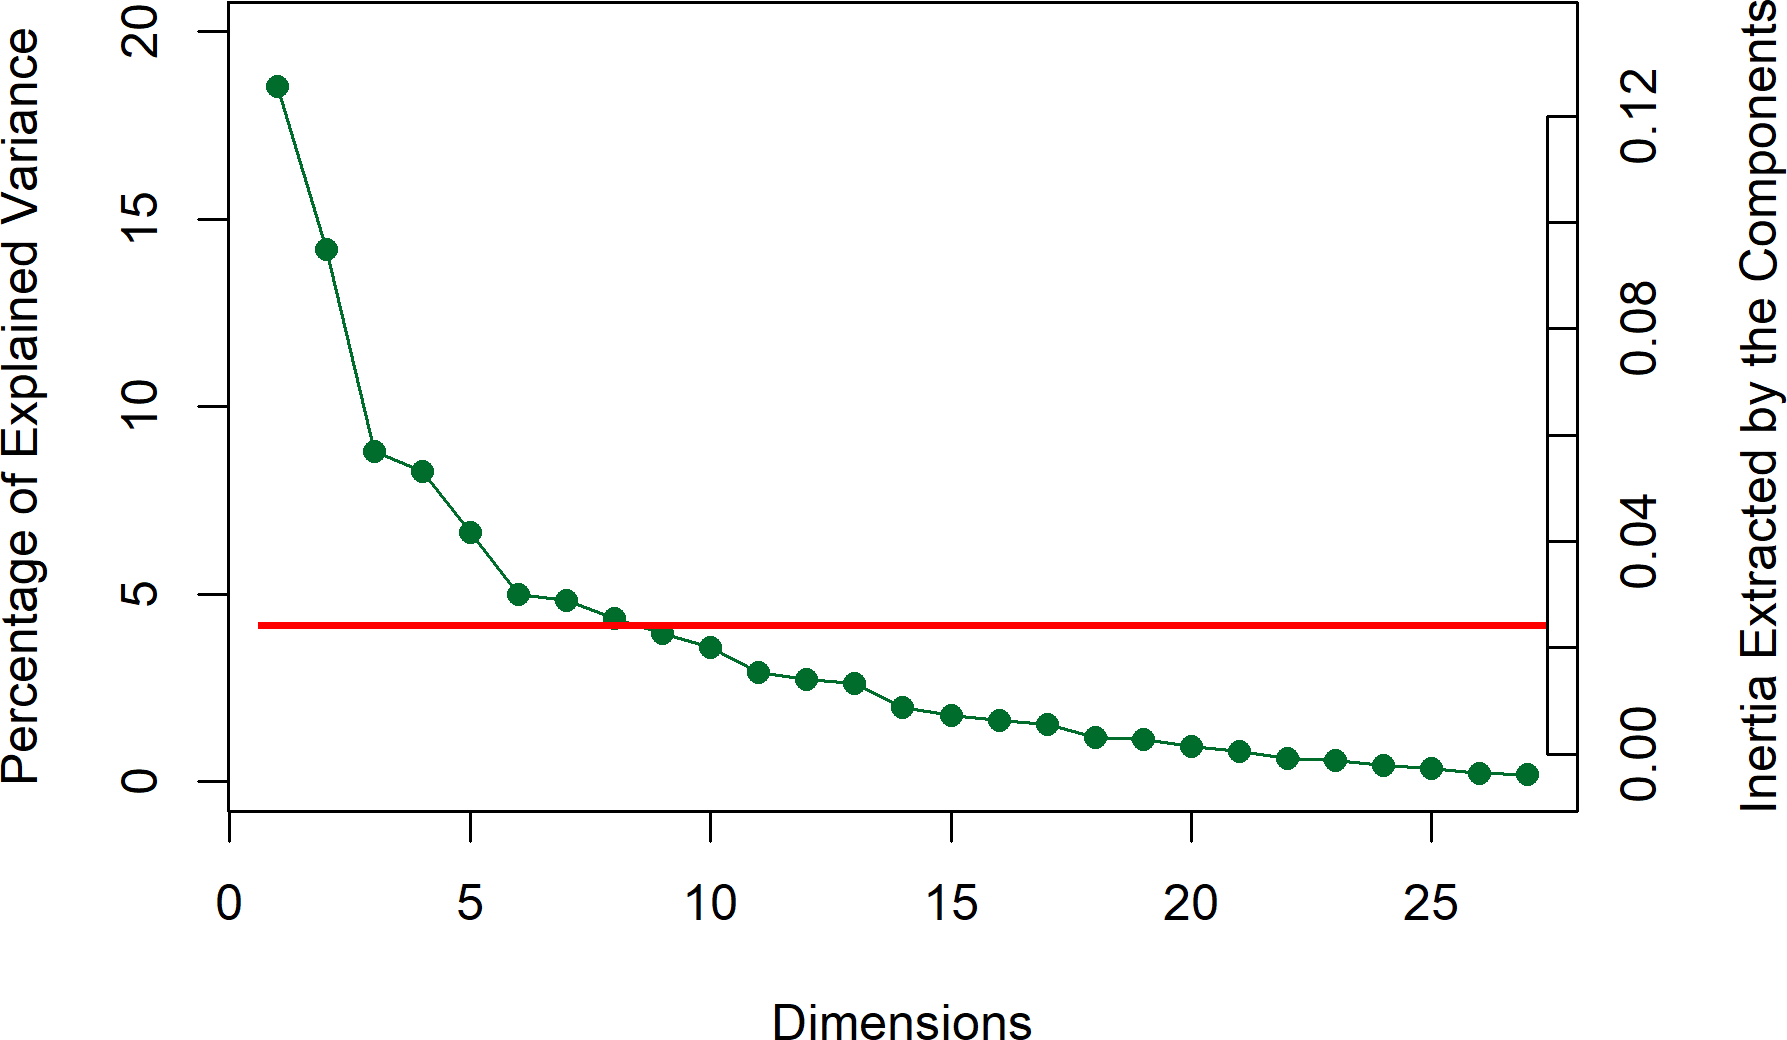
\includegraphics{./Music-Descriptor-Space_files/figure-latex/scree4excerptsq-1.png}
  \caption{ }\label{fig:scree4excerptsq}  
 \end{center}
\end{wrapfigure}

The results of the CA performed on the contingency table revealed two significant dimensions, accounting for 32.74\% of the total variance. Figure \ref{fig:scree4excerptsq} displays the scree plot, which shows for this analysis the percentage of variance explained by each dimension.

Preliminary plots of the factor scores obtained from the CA revealed that Excerpts 6 and 14 distorted the factor space, with these two excerpts dominating the second and third dimensions, respectively. To help interpret the factor space, these two excerpts were removed from the data and the CA was recomputed. Excerpts 6 and 14 were then added back in as \emph{supplementary observations}, a technique which visualizes the information these elements share with the other elements in the sample without distorting the factor space.

The HCA revealed four clusters (see supplementary materials for the dendrogram). Figure \ref{fig:factormapsQ}a displays these clusters represented by colors, with Excerpts 6 and 14 as supplementary observations colored separately. Figure \ref{fig:factormapsQ}b displays the qualities, colored by variable. To avoid overcrowding, only the levels of qualities that contributed significantly (see below, and Figure \ref{fig:contributionsQ}) are shown. The space for the two plots is the same, but they are displayed separately here for ease of comparison and interpretation.

The distance between any two points on a single plot in Figure \ref{fig:factormapsQ} can be interpreted directly as similarity, but the distance between points on separate plots cannot. Instead, the angle between an excerpt (left) and a quality (right) indicates their correlation. An angle of 0 or 180 degrees indicates a perfect positive or negative correlation, respectively, and an angle of 90 degrees indicates no correlation --- the two items share no information. See Abdi and Williams (2010) for a more in-depth discussion.

\begin{figure}

{\centering 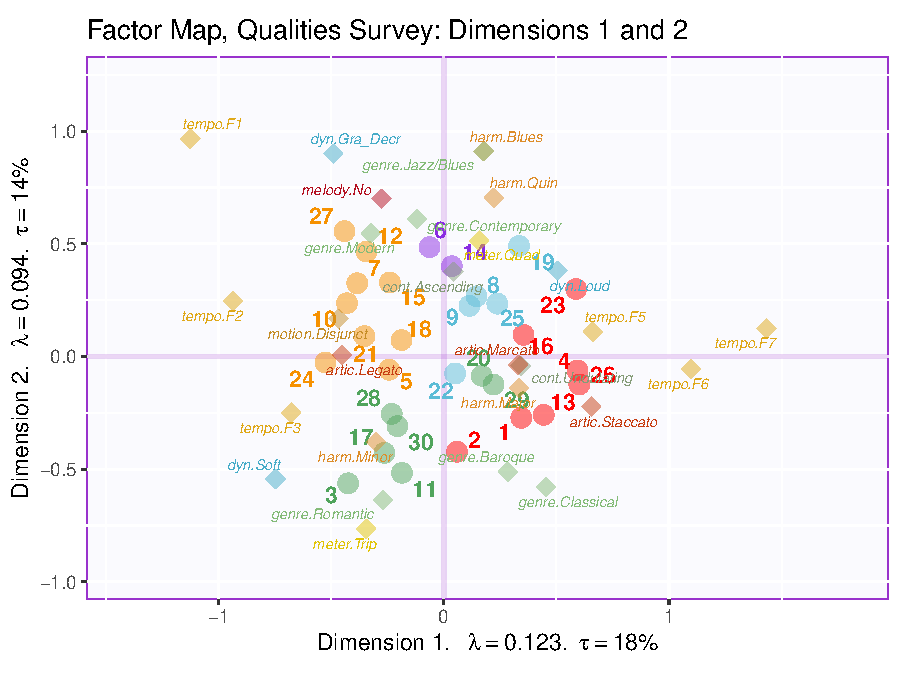
\includegraphics{Music-Descriptor-Space_files/figure-latex/factormapsQ-1} 

}

\caption{ }\label{fig:factormapsQ}
\end{figure}

To evaluate the relative importance of the excerpts and musical qualities in defining each dimension, we computed the \emph{contributions} of the excerpts and qualities to the factorial dimensions. Contributions are similar to a squared coefficient of correlation. They vary between zero and one with zero indicating no importance and one indicating maximum importance (Abdi \& Williams, 2010). Contributions --- being square --- are always positive, and to facilitate interpretation the contributions are signed in Figure \ref{fig:contributionsQ} to reflect the sign of the factor scores of the excerpts or qualities. Contributions larger than the average contribution are traditionally considered important to interpret factorial dimensions. A plot featuring showing contributions for all of the variables can be found in supplementary materials.

Figure \ref{fig:contributionsQ} shows the excerpts and qualities relevant for interpretation of the first two dimensions. Contributing positively to Dimension 1 are Excerpts 4, 13, 23, and 26, and contributing negatively are Excerpts 3, 7, 10, 24, and 27. Tempo, articulation, and dynamics seem to define the first dimension.

Dimension 1 separates the levels of the tempo variable from low (tempo.F2 and tempo.F1) in the negative direction to high (tempo.F6 and tempo.F7) in the positive direction. This dimension also separates articulations legato (smooth) from marcato and staccato (accented and separate), and dynamics soft to loud in the same way, negative to positive. Single levels from other variables also contribute to the first dimension: major harmony, triple meter, classical genre, undulating contour, and disjunct motion.

The second dimension features important contributions from the levels of the dynamics, genre, harmony and meter variables. Single levels of other variables also contribute to this dimension, namely slow tempo, ascending contour, and ``no melody.'' Dimension 2 separates Excerpts 2, 3, 11, and 17 in the negative dimension from Excerpts 7, 12, 15, 27, and 19 in the positive direction. A full enumeration of contributions and bootstrap ratios is available at the URL in the author note.

\begin{figure}

{\centering 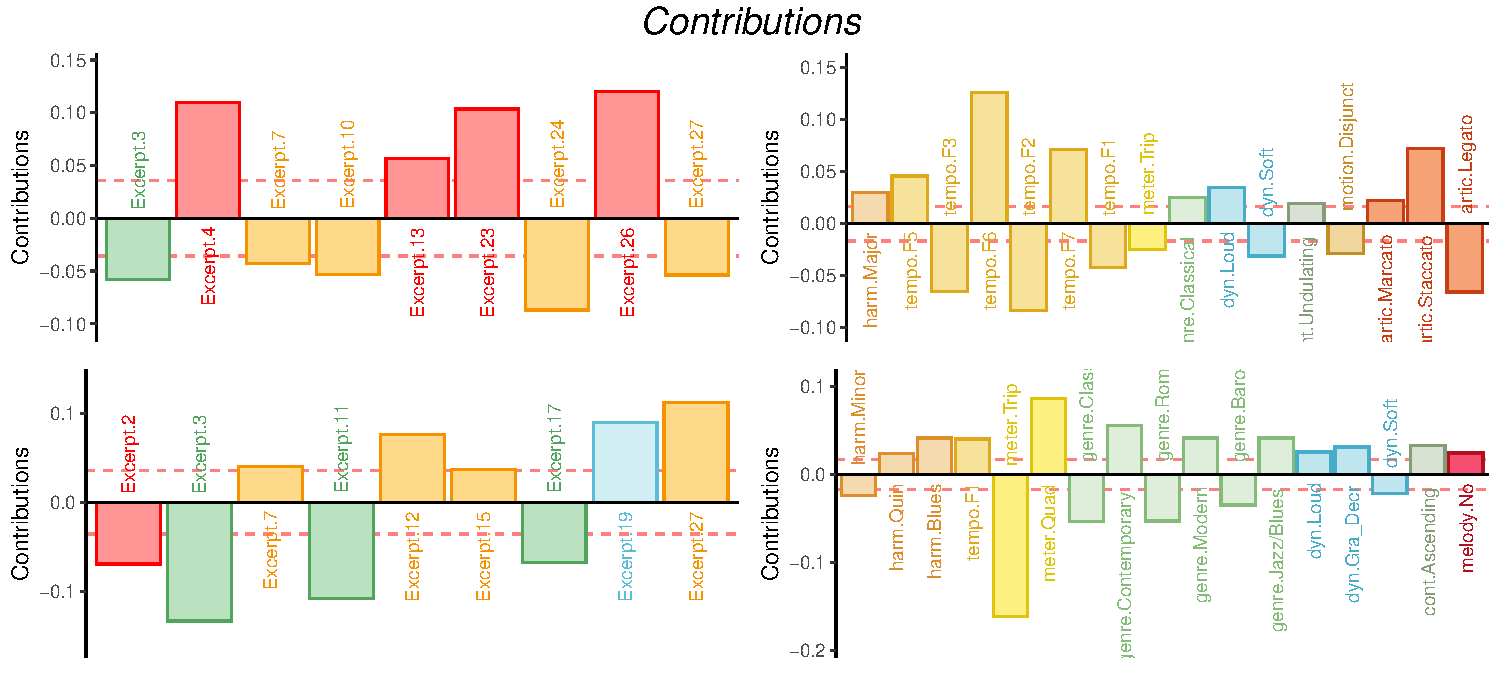
\includegraphics{Music-Descriptor-Space_files/figure-latex/contributionsQ-1} 

}

\caption{ }\label{fig:contributionsQ}
\end{figure}

\hypertarget{discussion}{%
\subsection{Discussion}\label{discussion}}

There are a few musical connections revealed in Figure \ref{fig:factormapsQ}. The connection between tempo and articulation is apparent, as is the connection between genre and harmony (Cohn et al., 2001). Staccato articulations, correlated on this factor plot with high tempos, are played light and separate, and legato articulations, correlated with slow tempos, are played smooth and connected. In terms of performance practice, slow and long notes are played in a legato style to create a sense of continuity, and fast moving notes or phrases do not require the same technique. The coordinate mapping of jazz/blues harmony and genre, which are stacked right on top of one another is the most extreme example of a genre being associated with certain harmonic material, but other connections are also revealed. The second dimension separates the older styles, such as baroque, classical, and romantic, from the newer styles, impressionist, modern, and contemporary. Dimension 2 associates the simpler harmonies of major and minor and the more complex harmonies of chromatic, whole tone, quintal, blues, and ambiguous with older and newer styles, respectively, following historical practice. The Classical era had fairly structured rules for both harmony and voice leading, but the Romantic era relaxed those rules and introduced more complex harmonies (Cohn et al., 2001). The gradual devolution of those rules and the increase in complexity of harmony continued through the modern and contemporary styles (Cohn et al., 2001; Kennedy et al., 2013).

These musical connections facilitate our interpretation of the first two dimensions. The first dimension can be interpreted as arousal --- tempo, articulation, and dynamics all load from greater arousal to lesser on the first dimension. Dimension 2 is less clear, and does not seem to be tied to valence. Minor and major harmony, for example, both score negatively on Dimension 2. Instead, Figure \ref{fig:contributionsQ} shows that while two levels of the meter variable are the most important for this dimension, that genre is also important, based on the number of levels of genre that contribute significantly to Dimension 2.

Genre as a defining element for the second dimension is also supported by the story of Excerpts 6 and 14. As stated above, the HCA initially revealed 6 clusters, with Excerpts 6 and 14 each in their own cluster. This may be because these two excerpts were the sole representatives of their respective genres. Excerpt 6 is minimalist, à la Steve Reich, and Excerpt 14 is jazzy. Removing these two from the dataset and recomputing the CA and the HCA did not change the clusters for the rest of the excerpts, suggesting that the other Excerpts are in stable groups.

Finally, we note that because of the nature of this survey, these results tell us more about the excerpts themselves rather than the behavior of the participants. The participants rated the stimuli similarly, validating the variety among the excerpts, indicating that they are different enough to create a large and varied factor space.

\hypertarget{experiment-2-musical-adjectives-survey}{%
\section{Experiment 2: Musical Adjectives Survey}\label{experiment-2-musical-adjectives-survey}}

\hypertarget{methods-1}{%
\subsection{Methods}\label{methods-1}}

\hypertarget{participants-2}{%
\subsubsection{Participants}\label{participants-2}}

Participants with self-reported normal hearing were recruited for Experiment 2 without regard to level of music training. Participants in the United States were recruited through the UT Dallas Psych Research Sign-up (SONA) System and by word of mouth and social media. French participants were recruited by word of mouth, email, and social media. Only participants who signed up via the SONA System were compensated with research participation credit, other participants were not compensated in any way. Of a total 520 survey responses, 160 were removed for being incomplete, leaving a total of 360. Additionally, participants from the US who indicated a nationality other than American were excluded from analysis. ``Ghanian,'' for example, was not included, but responses such as ``Asian-American'' were. This left a total of 279 (\(\textit{N}_F\) = 108, \(\textit{N}_A\) = 171) survey responses for analysis. All recruitment measures were approved by the UT Dallas IRB.

\hypertarget{stimuli-1}{%
\subsubsection{Stimuli}\label{stimuli-1}}

The stimuli used for Experiment 2 are the same as those used for Experiment 1.

\hypertarget{survey-1}{%
\subsubsection{Survey}\label{survey-1}}

The procedure for participants in Experiments 1 and 2 was similar. They received a link to a Qualtrics survey presented in either English or French, depending on their location, and instructions regarding listening environment were the same. After standard informed consent procedures, the participants listened to 15 of the 30 excerpts, presented one at a time, in a random order, and performed a CATA task. The task was to evaluate the stimuli using thirty-three adjectives such as `dark,' `warm,' and `colorful' (French: `sombre,' `chaleureux,' and `colore'). The adjectives for the AS were selected using Wallmark (2019) as a guide and in consult with a French professional musician. Some adjectives were initially selected in French and some in English. In all cases, adjectives were selected for which there was a clear French (vis-à-vis English) translation. The adjectives are listed in English and in French in the supplementary materials. Following the experimental task, the participants were asked to provide demographic data, including age, gender identity, nationality, occupation, and musical experience.

\hypertarget{data-processing-analysis}{%
\subsubsection{Data Processing \& Analysis}\label{data-processing-analysis}}

Data for the survey for Experiment 2 (Adjectives survey/AS) were processed similarly to those for Experiment 1. To process the data, first, all French survey responses were translated into English. Both sets of responses were then converted into ``bricks'' of data, with the excerpts on the rows, the adjectives on the columns, and participants on the pages. On any page, at the intersection of any row and column was a one or a zero, with a one indicating that this participant had selected this adjective (column) to describe this stimulus (row). The bricks were then concatenated and summed across pages to obtain a pseudo-contingency table in which the intersection of a row and a column was the total number participants who selected an adjective to describe an excerpt.

After data processing, the data were in two usable forms, a brick and a contingency table. To analyze the similarity structure between participants, we computed a co-occurrence matrix from the brick with participants on the rows and columns, such that the intersection of a row and column represented the number of similar choices between participants. This was then analyzed using MDS.

To analyze the excerpts and adjectives and obtain the music quality space, we performed a CA on the contingency table. To identify potential clusters of excerpts or adjectives, two separate HCAs were computed, one each on the row factor scores (excerpts) and the column factor scores (adjectives) obtained from the CA.

We used MFA to explore the differences between the ratings of French and American participants. To prepare the data, we summed separate pseudo-contingency tables for the French and American participants, with the excerpts on the rows and the adjectives on the columns. Because MFA does not evaluate rows and columns in the same analysis the way the CA does, we had to transpose each of these tables to obtain tables with the adjectives on the rows and the excerpts on the columns. The two pairs of tables were concatenated and we then ran separate MFAs on these.

\hypertarget{results-1}{%
\subsection{Results}\label{results-1}}

\hypertarget{participants-3}{%
\subsubsection{Participants}\label{participants-3}}

%\begin{wrapfigure}{h}{.5\textwidth}  
%  \begin{center}
%    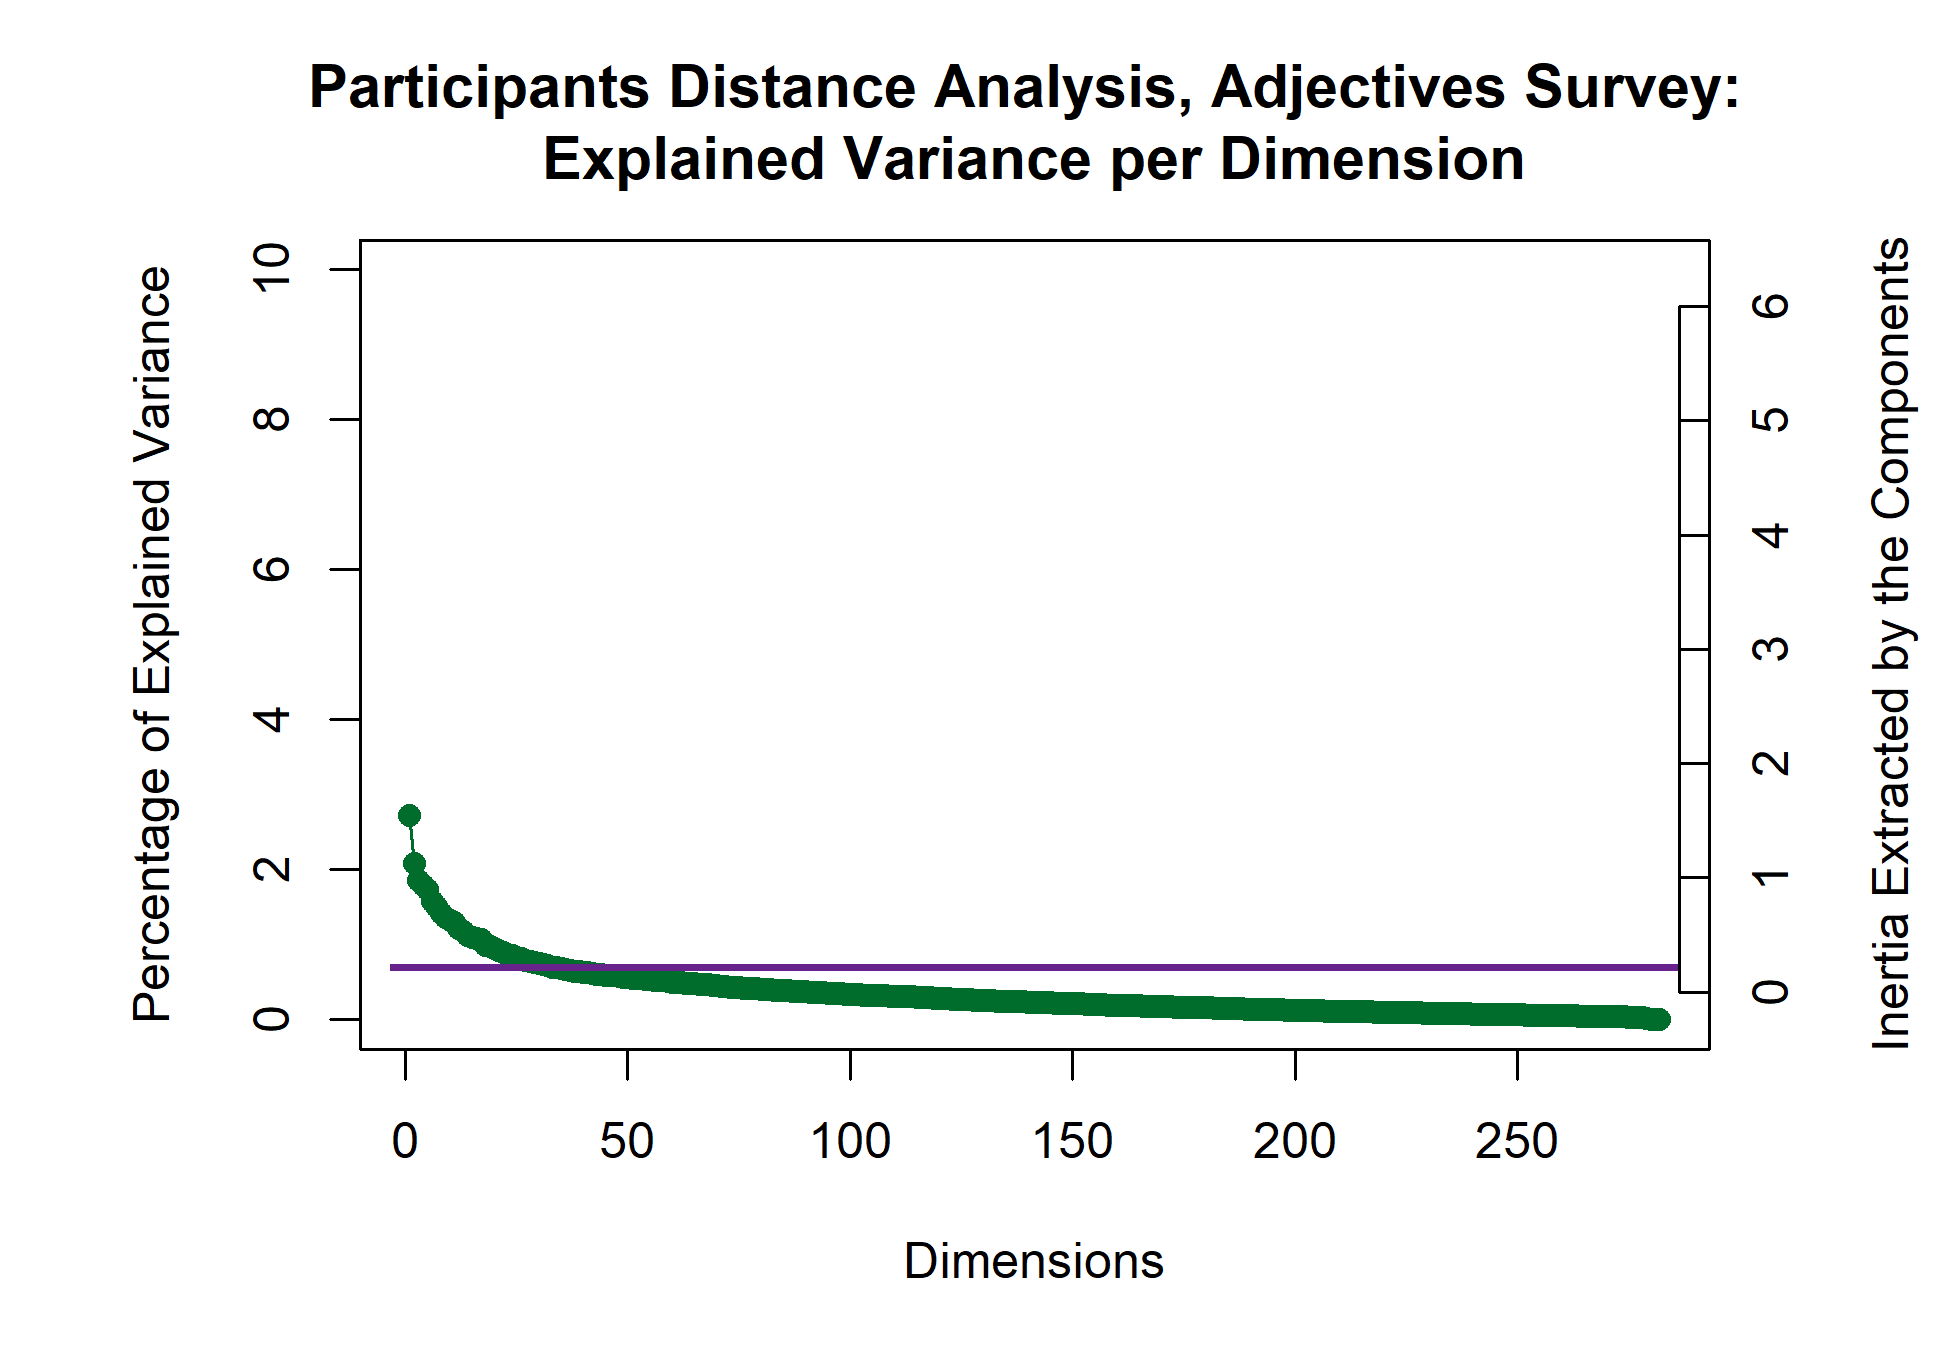
\includegraphics{./Music-Descriptor-Space_files/figure-latex/a.part.scree-1.png}
%  \caption{ }\label{fig:apartscree}  
% \end{center}
%\end{wrapfigure}

The MDS performed on the co-occurence matrix revealed significant differences between the French and American participants, \(\textit{p}\). \textless{} .01. The factor scores, with group means and bootstrap-derived confidence intervals of the participants are plotted in Figure \ref{fig:map4RVA}. Additional analyses using gender identity and level of music training as factors were not found to be significant.

\begin{figure}   
  \centering  
  \caption{${R_V}$ Analysis of Participants in the Adjectives Survey}
    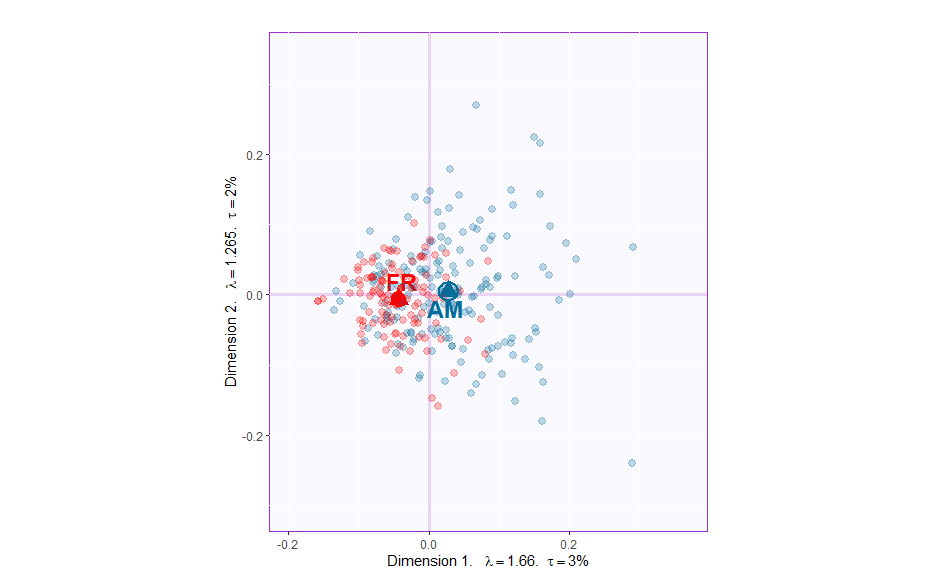
\includegraphics[width=0.7\columnwidth]{./Music-Descriptor-Space_files/figure-latex/apartrvmap.png}
  \label{fig:map4RVA}
  \caption*{\footnotesize \textit{Note.}  Group means are indicated with triangles and labled with AM and FR. The ellipse around the group mean indicates the confidence interval, after bootstrapping 1000 iterations. The fact that there is a clear separation between the group means and the confidence intervals suggests that there is a significant difference between the groups, \textit{p} > .001.}
\end{figure}

\hypertarget{excerpts-1}{%
\subsubsection{Excerpts}\label{excerpts-1}}

The CA performed on the AS pseudo-contingency table revealed two significant dimensions, accounting for 72.45\% of the variance total variance. Figure \ref{fig:scree4excerptsq} displays the scree plot, which shows for this analysis the percentage of variance explained by each dimension. Although excerpts 6 and 14 were removed from Experiment 1 data for being outliers, they were not outliers in this analysis, and were therefore included in all of the analyses for Experiment 2.

\begin{wrapfigure}{h}{.5\textwidth}  
  \begin{center}
    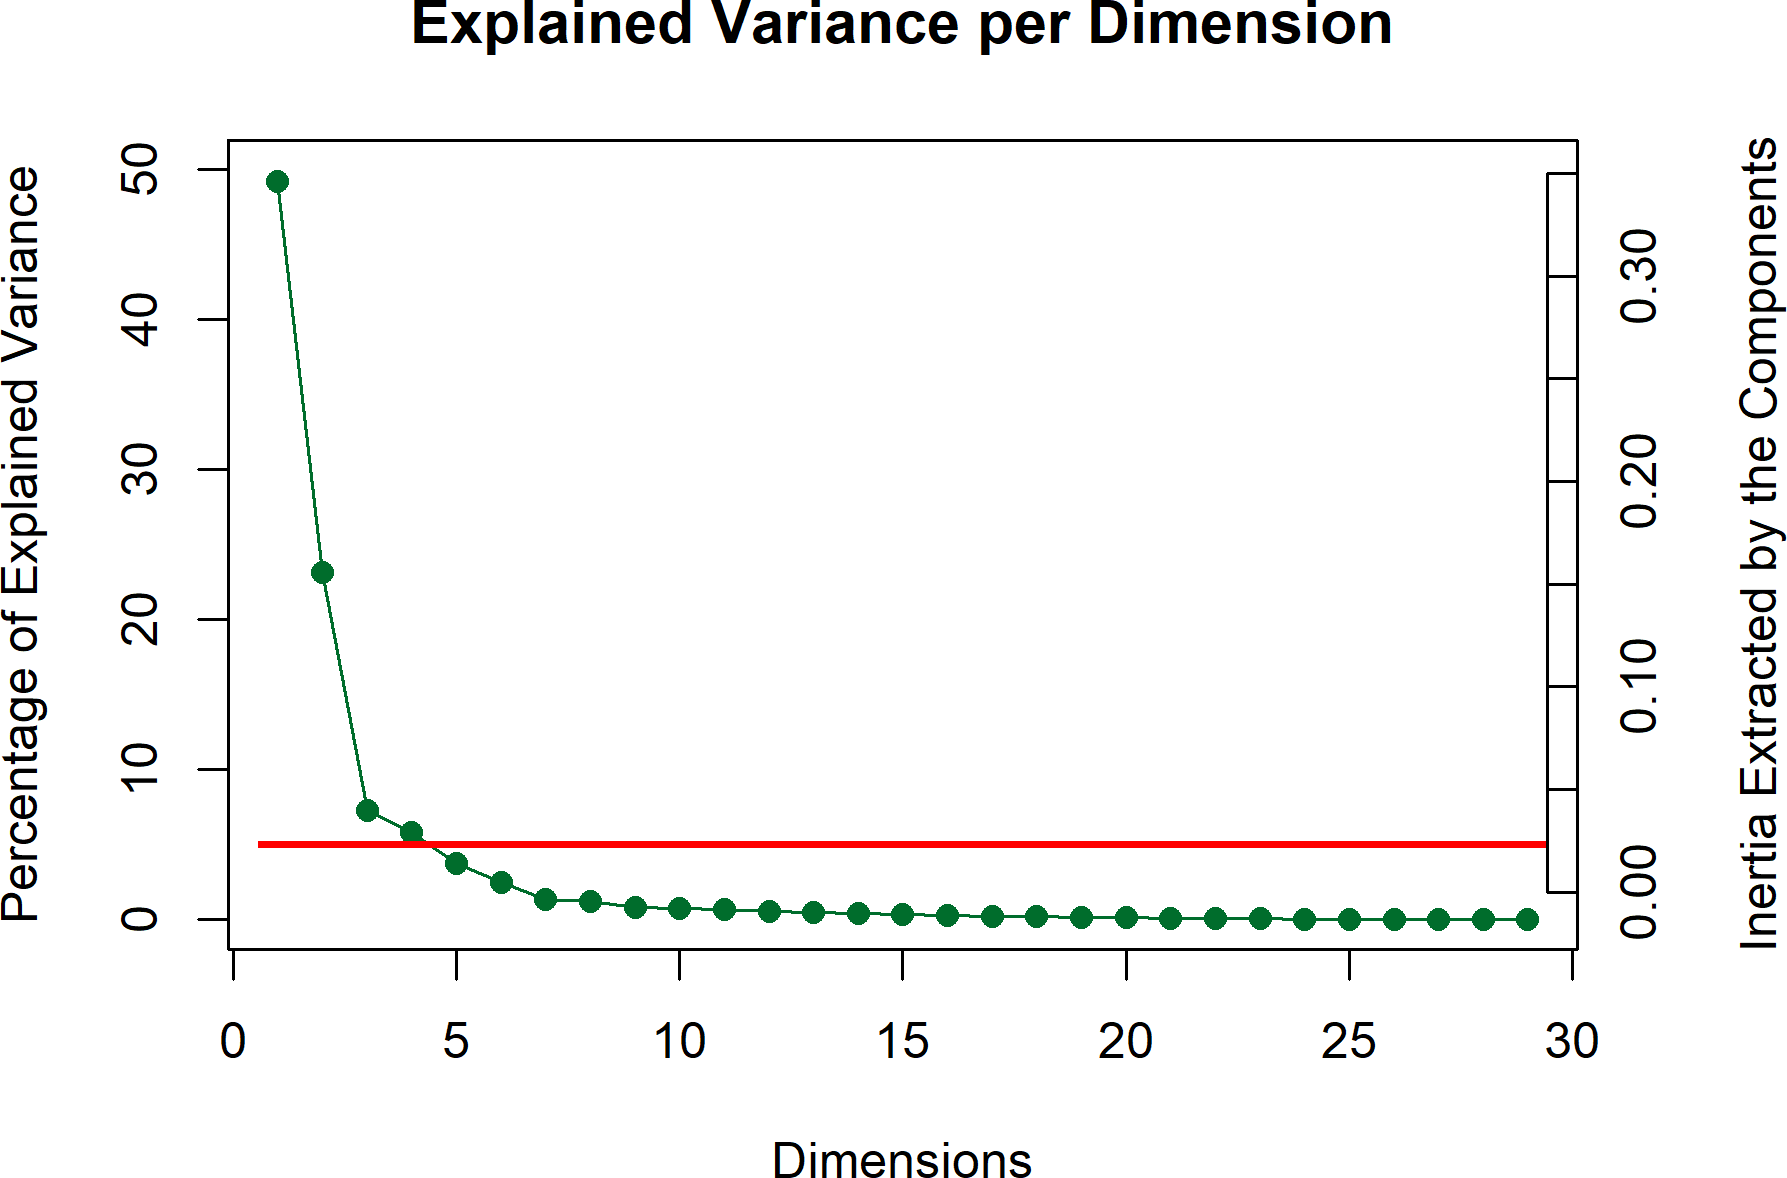
\includegraphics{./Music-Descriptor-Space_files/figure-latex/scree4descriptors-1.png}
  \caption{ }\label{fig:scree4descriptors}  
 \end{center}
\end{wrapfigure}

\begin{figure}   
  \centering  
  \caption{Symmetric Plots for Rows and Columns of the Adjectives Surveys, by Participant Nationality}
    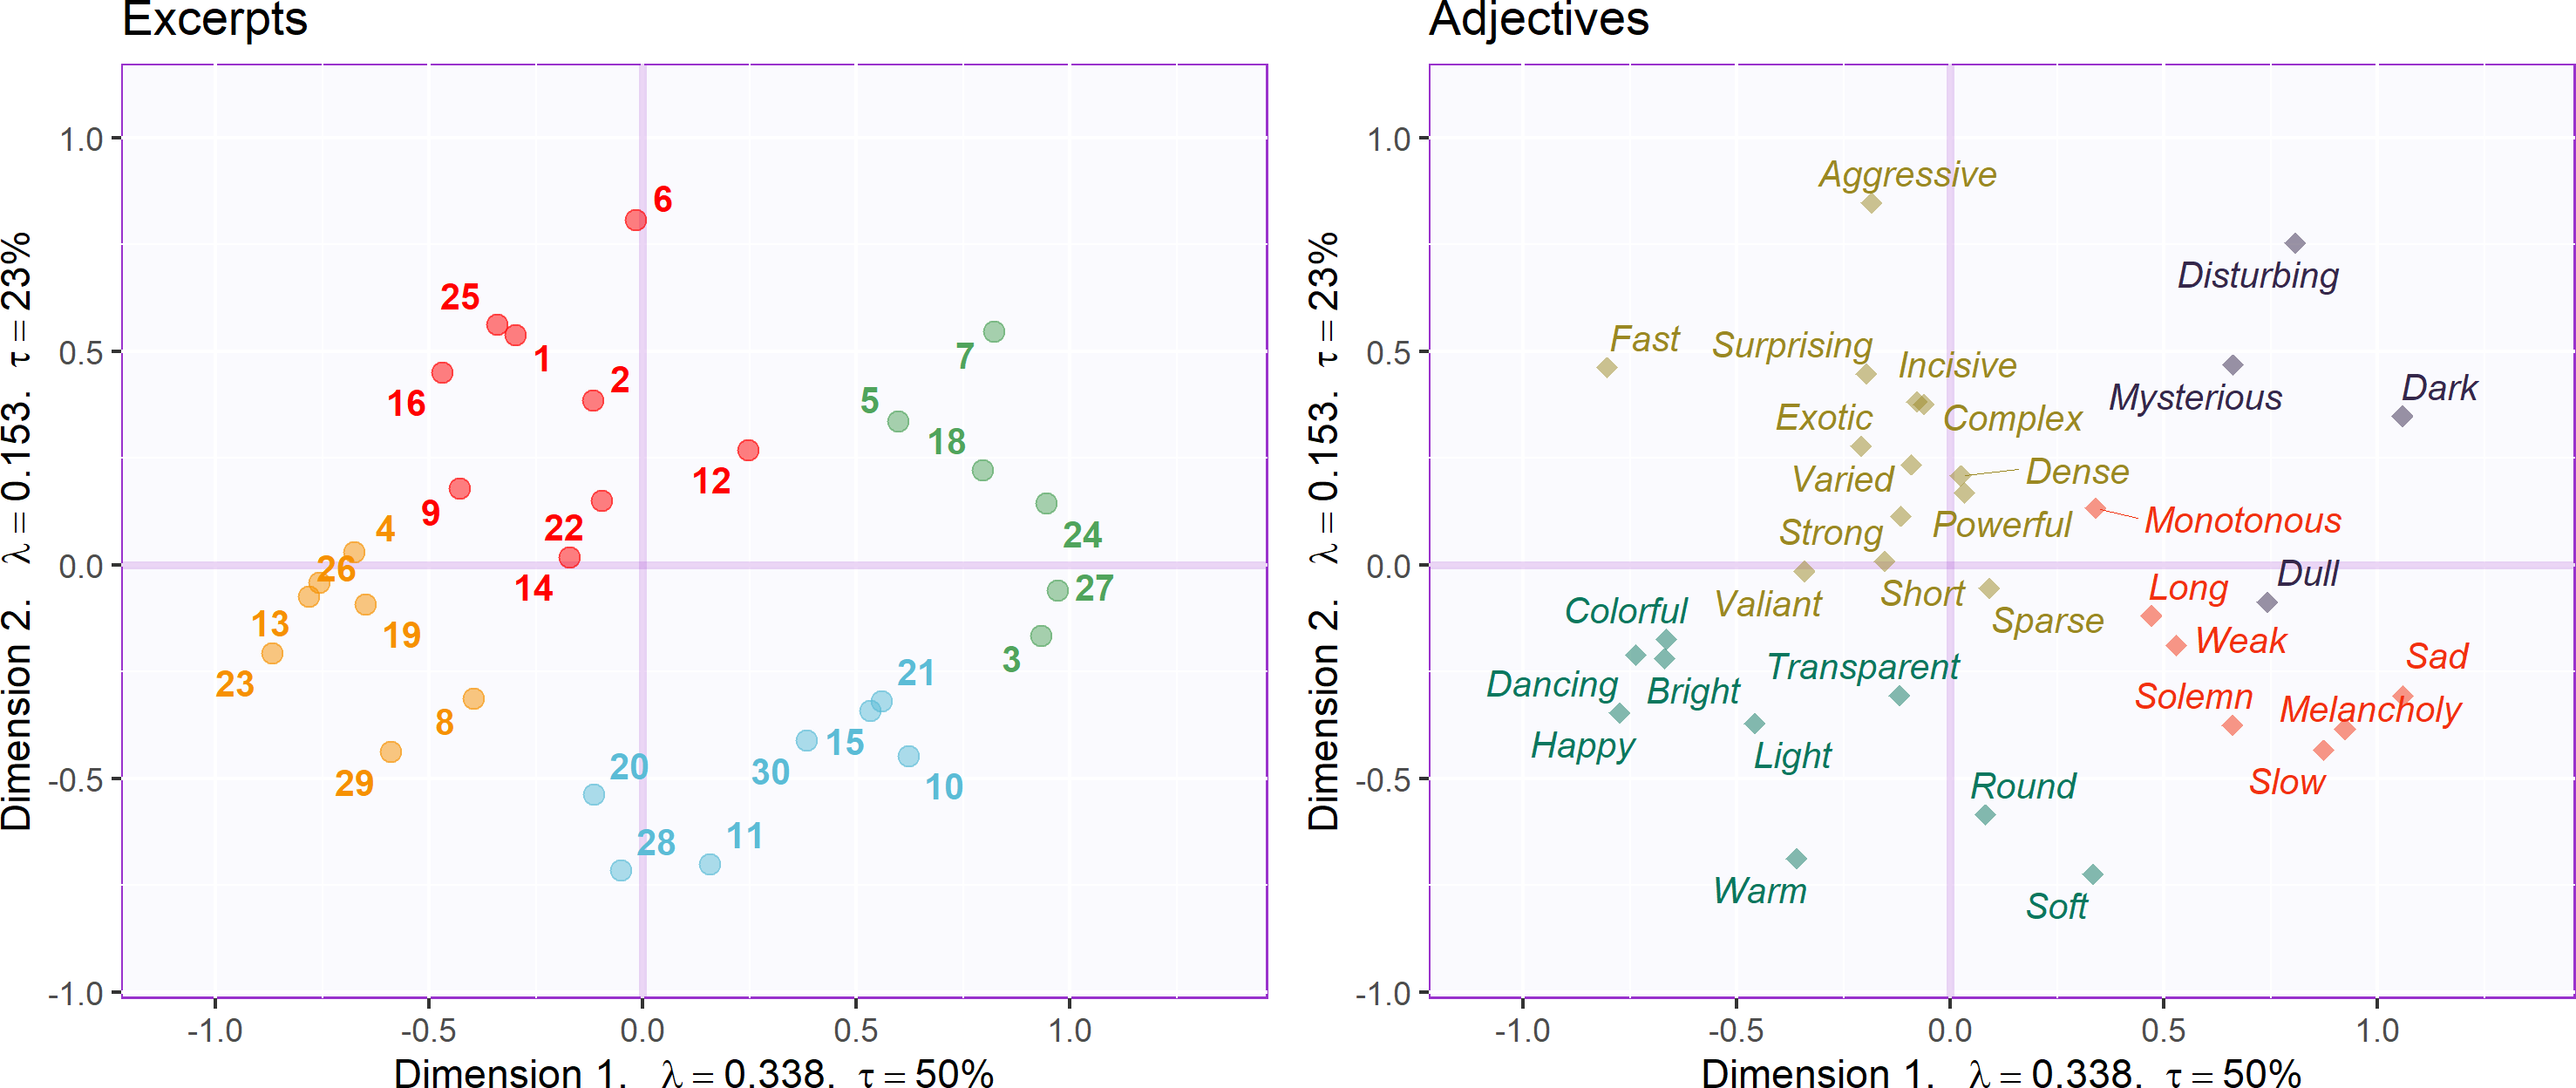
\includegraphics{./Music-Descriptor-Space_files/figure-latex/factormapsA-1.png}
  \label{fig:factormapsA}
  \caption*{\footnotesize \textit{Note.}  This plot shows the row and column factor scores displayed separately. The constraints, or the space for the plot are the same between both plots. They are displayed this way to avoid overcrowding between the rows and columns.}
\end{figure}

The HCAs computed separately on the row and column factor scores revealed four clusters for each, and the excerpts and adjectives are colored according to those clusters in Figure \ref{fig:factormapsA}. This figure displays the row (excerpt) and column (adjective) factor scores obtained from the CA computed on the AS contingency table. As with the factor plots for Experiment 1, the distance between any two points on the same plot can be interpreted directly as similarity, but the distance between points on separate plots cannot. Instead, the angle between an excerpt (left) and an adjective (right) indicates their correlation. An angle of 0 or 180 degrees indicates a perfect positive or negative correlation, respectively, and an angle of 90 degrees indicates no correlation --- the two items share no information. See Abdi and Williams (2010) for a more in-depth discussion.

The excerpts and variables important to interpretation of the first two dimensions obtained by the CA, are depicted in Figure \ref{fig:contributionsA}. Excerpts and variables are colored according to the clusters extracted from their respective HCAs. Dimension 1 features greater than average contributions from Excerpts 3, 5, 7, 10, 18, 24, and 27, in the positive direction and Excerpts 4, 13, 19, 23, 26, and 29 in the negative direction. Likewise, adjectives that contribute more than the average to the first dimension are ``Sad,'' ``Dark,'' ``Melancholy,'' ``Slow,'' ``Mysterious,'' ``Solemn,'' and ``Disturbing'' in the positive direction and ``Fast,'' ``Happy,'' ``Dancing,'' ``Colorful,'' and ``Bright'' in the negative direction.

On the second dimension, excerpts with important contributions in the positive direction are 1, 6, 7, 16, and 25, and in the negative direction are Excerpts 10, 11, 20, 28, and 29. The columns with contributions in the positive direction are ``Aggressive,'' ``Fast,'' ``Disturbing,'' ``Mysterious,'' ``Surprising'' and ``Complex,'' and those contributing important negative contributions are ``Warm,''Soft``,''Happy``,''Slow``,''Round``, and''Light".

Figure \ref{fig:mfasbs} displays partial factor score plots (see ``Multiple Factor Analysis'' above) of the results of the MFA evaluating the differences in rating behavior between French and American participants. Although the specific magnitudes of the dimensions extracted by the MFAs are different, as evidenced by the percentage of variance extracted (\(\tau\)) on the axes of the plots, the general space revealed by these analyses is similar to that revealed by the CA. Thus we can interpret the space similarly, relative to the valence-arousal plane. The triangles represent the compromise between the mental spaces of the French and American participants for each item, and the lines extending from the triangles indicate the partial factor scores for the items from the perspective of each group (Abdi et al., 2013). Excerpts and adjectives that were rated similarly have shorter lines extending from them, but excerpts that were rated differently have much longer lines. Examples of excerpts that were rated differently are numbers 6, 8, 12, and 17. Adjectives that were used differently include ``Disturbing,'' ``Round,'' ``Solemn,'' and ``Bright.''

\begin{figure}

{\centering 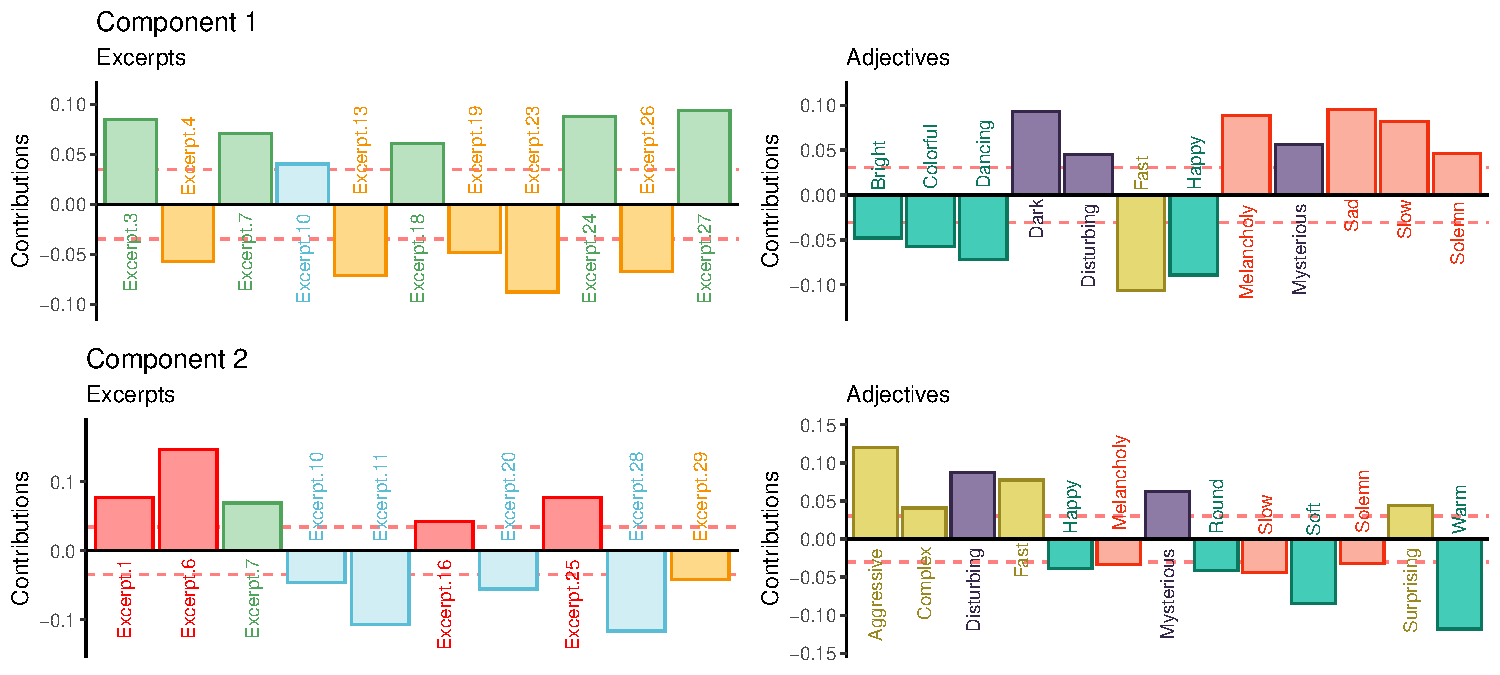
\includegraphics{Music-Descriptor-Space_files/figure-latex/contributionsA-1} 

}

\caption{ }\label{fig:contributionsA}
\end{figure}

\begin{figure}
     \centering
     \caption{Partial Factor Scores Plots from the MFA}
     \begin{subfigure}[b]{0.49\textwidth}
         \centering
         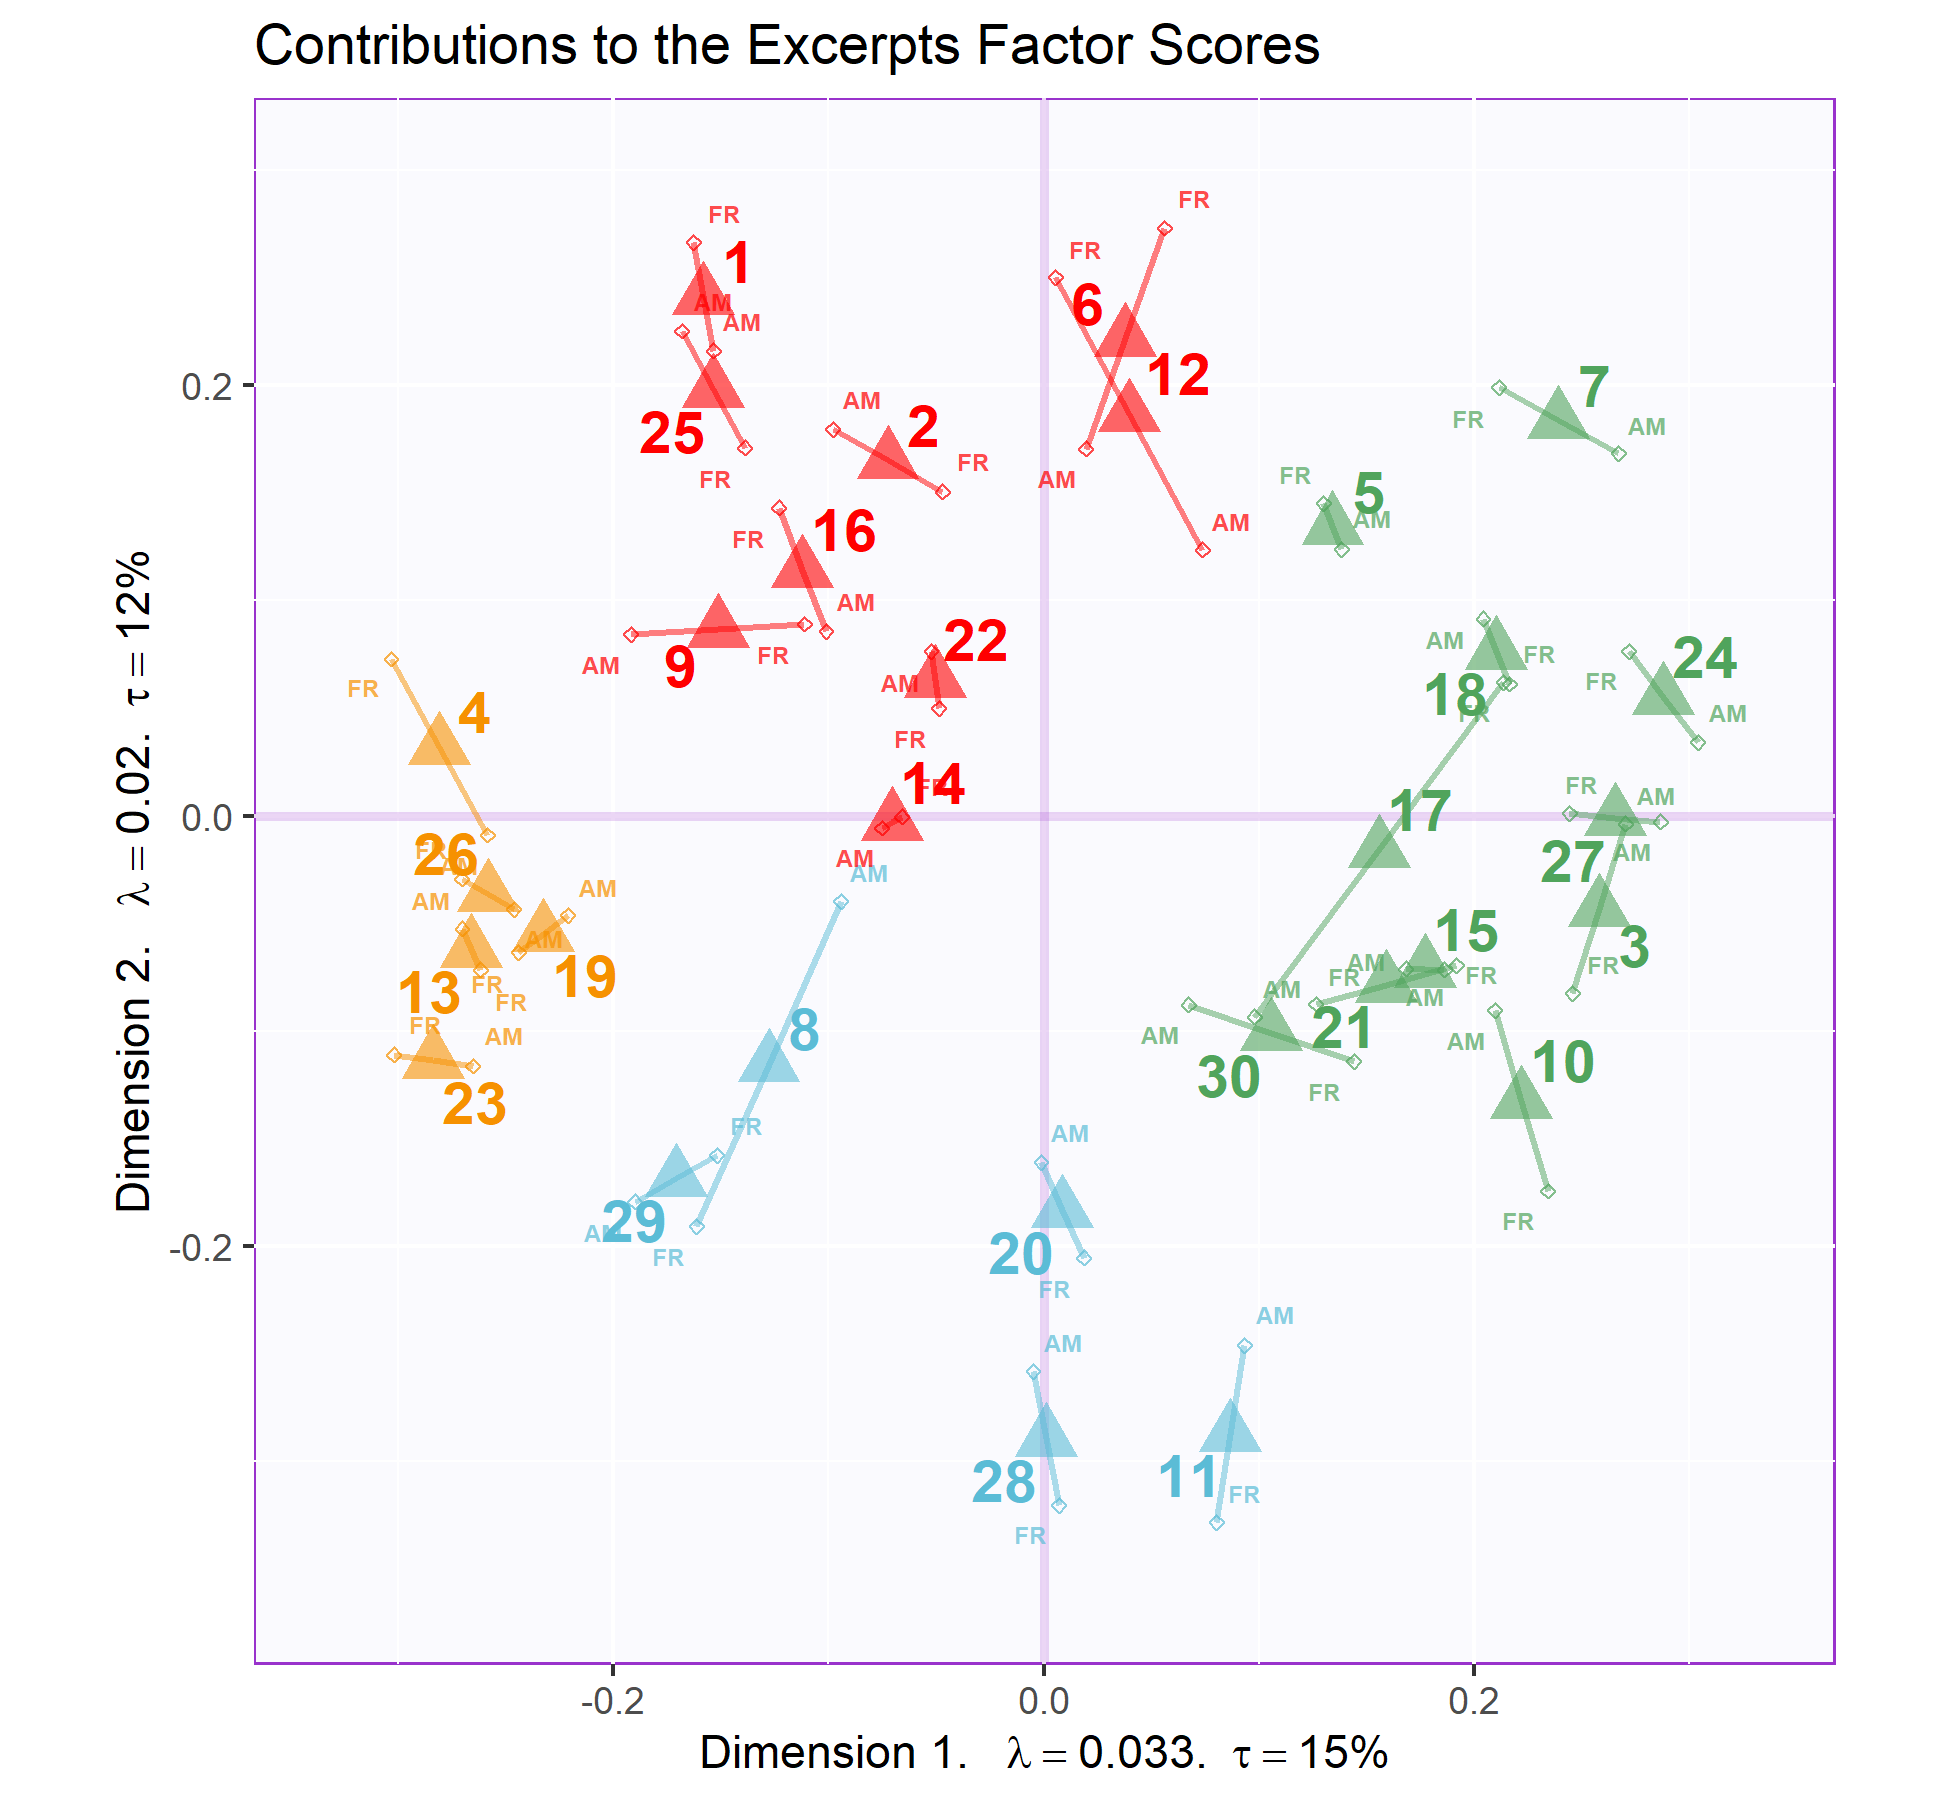
\includegraphics[width=\textwidth]{./Music-Descriptor-Space_files/figure-latex/mfasbs-1}
         %\caption{$y=x$}
         \label{fig:excerptspfs}
     \end{subfigure}
     \hfill
     \begin{subfigure}[b]{0.49\textwidth}
         \centering
         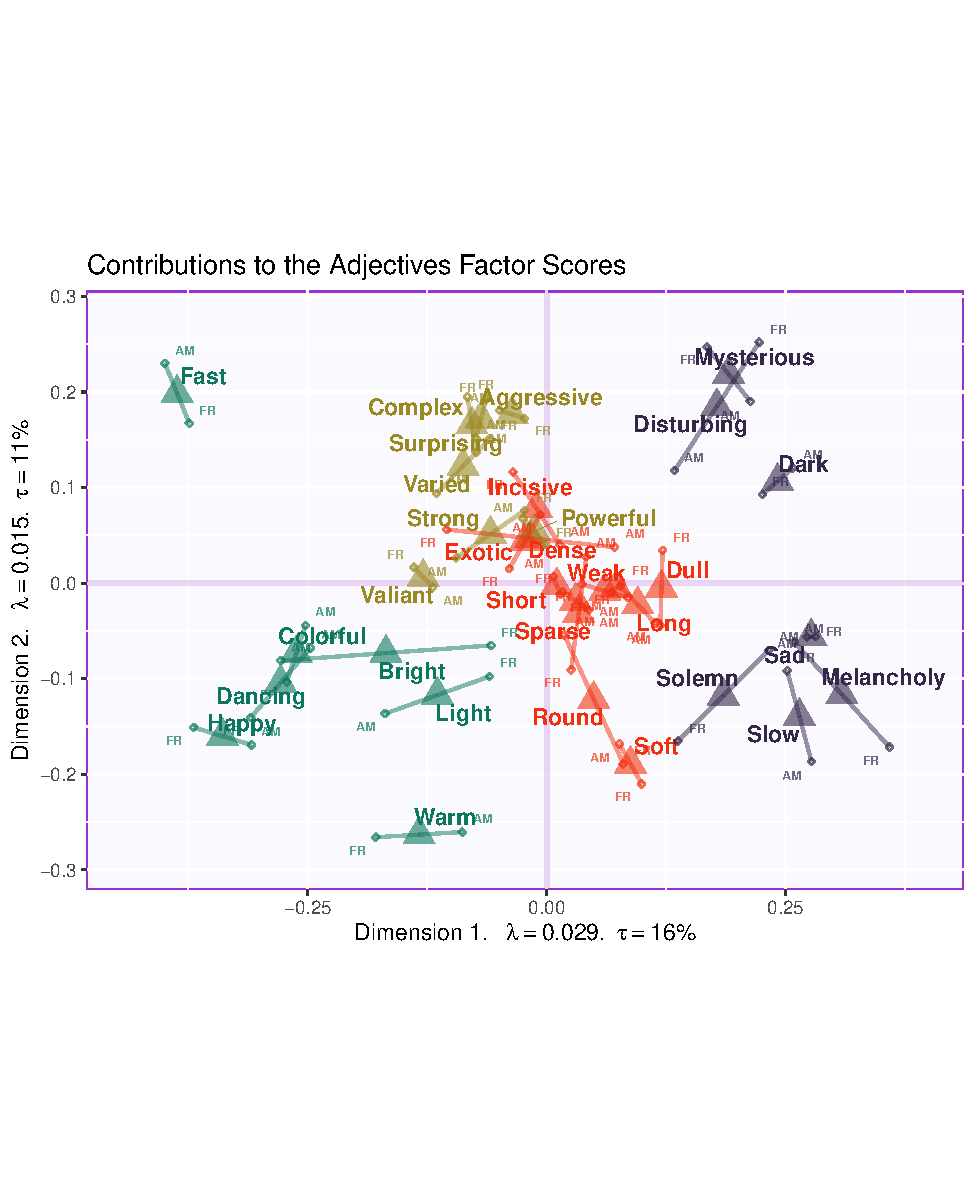
\includegraphics[width=\textwidth]{./Music-Descriptor-Space_files/figure-latex/mfasbs-2}
         %\caption{$y=3sinx$}
         \label{fig:adjectivespfs}
     \end{subfigure}
    \label{fig:mfasbs}
      \caption*{\footnotesize \textit{Note.}  In each plot, the triangles represent the combined factor scores and the small circles represent the partial factor scores contributed by each of the groups.}
\end{figure}

\hypertarget{discussion-1}{%
\subsection{Discussion}\label{discussion-1}}

Interpreting the differences in how the adjectives and the excerpts are distributed in the space is aided by considering the valence-arousal plane. Excerpt 17 may provide the best

One clear example is Excerpt 6, which is in the low valence/high arousal quadrant in the American plot, and the high valence/high arousal quadrant in the French plot, suggesting that the two groups tended to assign different valence to this excerpt. For the adjectives, `bright' and `dancing' are directly on top of one another in the American plot, but there is some space between the two in the French plot. This reflects shared meaning but differences in semantics or associations between languages.\\
Although this experiment was designed to evaluate the cognitive response to music, and not the emotional response, there is significant overlap in the results observed here and the results of the work investigating music and emotion, specifically in the appearance of the valence-arousal plane. Studies on music and emotion have used this construct as a way of measuring emotion, but the original proposal was that this plane is simply a measure of ``meaning'' (Osgood \& Suci, 1955). The adjectives selected for use in Experiment 2 reflect this original proposal, as they were selected specifically to represent a cognitive space, not an emotional one.

The valence-arousal plane revealed by the CA is also present here, and provides a framework for interpreting the differences between groups. Excerpt 17 is perhaps the most extreme example. American participants rated this excerpt with much lower arousal and slightly less negative valence than the French participants, so much so that for the American participants, the excerpt landed in the low arousal/negative valence quadrant, and for the French participants it landed in the high arousal/negative valence quadrant. Another interesting case is for Excerpt 8, which lands in the same quadrant for both groups, but much further from the origin for the French participants than the Americans.\\
Some examples of differences in the use of adjectives includes ``disturbing'' (inquiétant) seems to be more extreme for the French participants than the Americans. In English, ``Solemn'' (solennel) carries more valence, and in French it carries more arousal; similarly, ``bright'' (brillant) seems to carry much more positive valence in English than in French. In English, ``melancholy'' (melancolique) and ``sad'' (triste) were used the same, but in French they were used very differently.

\hypertarget{experiment-3-combined-surveys}{%
\subsection{Experiment 3: Combined Surveys}\label{experiment-3-combined-surveys}}

Experiment 3 used the pseudo-contingency tables from both Experiments 1 and 2. Since excerpts 6 and 14 were excluded from analysis for Experiment 1, those rows were also removed from the contingency table for Experiment 2. This is so that the dimensions of the two tables for this PLSC would be conformable. The goal of this experiment was to identify the strongest shared signal between the two tables. Remember that PLSC shows what is common between two different sets of data --- how often an excerpt was associated with \emph{both} a musical quality and an adjective. The visualizations below show which adjectives are associated with which musical dimensions. Even though both individual tables have their own factor spaces, plotting the common factor space between the two should allow us to see which excerpts are separated from one another using data from both surveys.

\hypertarget{results-2}{%
\subsubsection{Results}\label{results-2}}

\begin{wrapfigure}{h}{.5\textwidth}  
  \begin{center}
    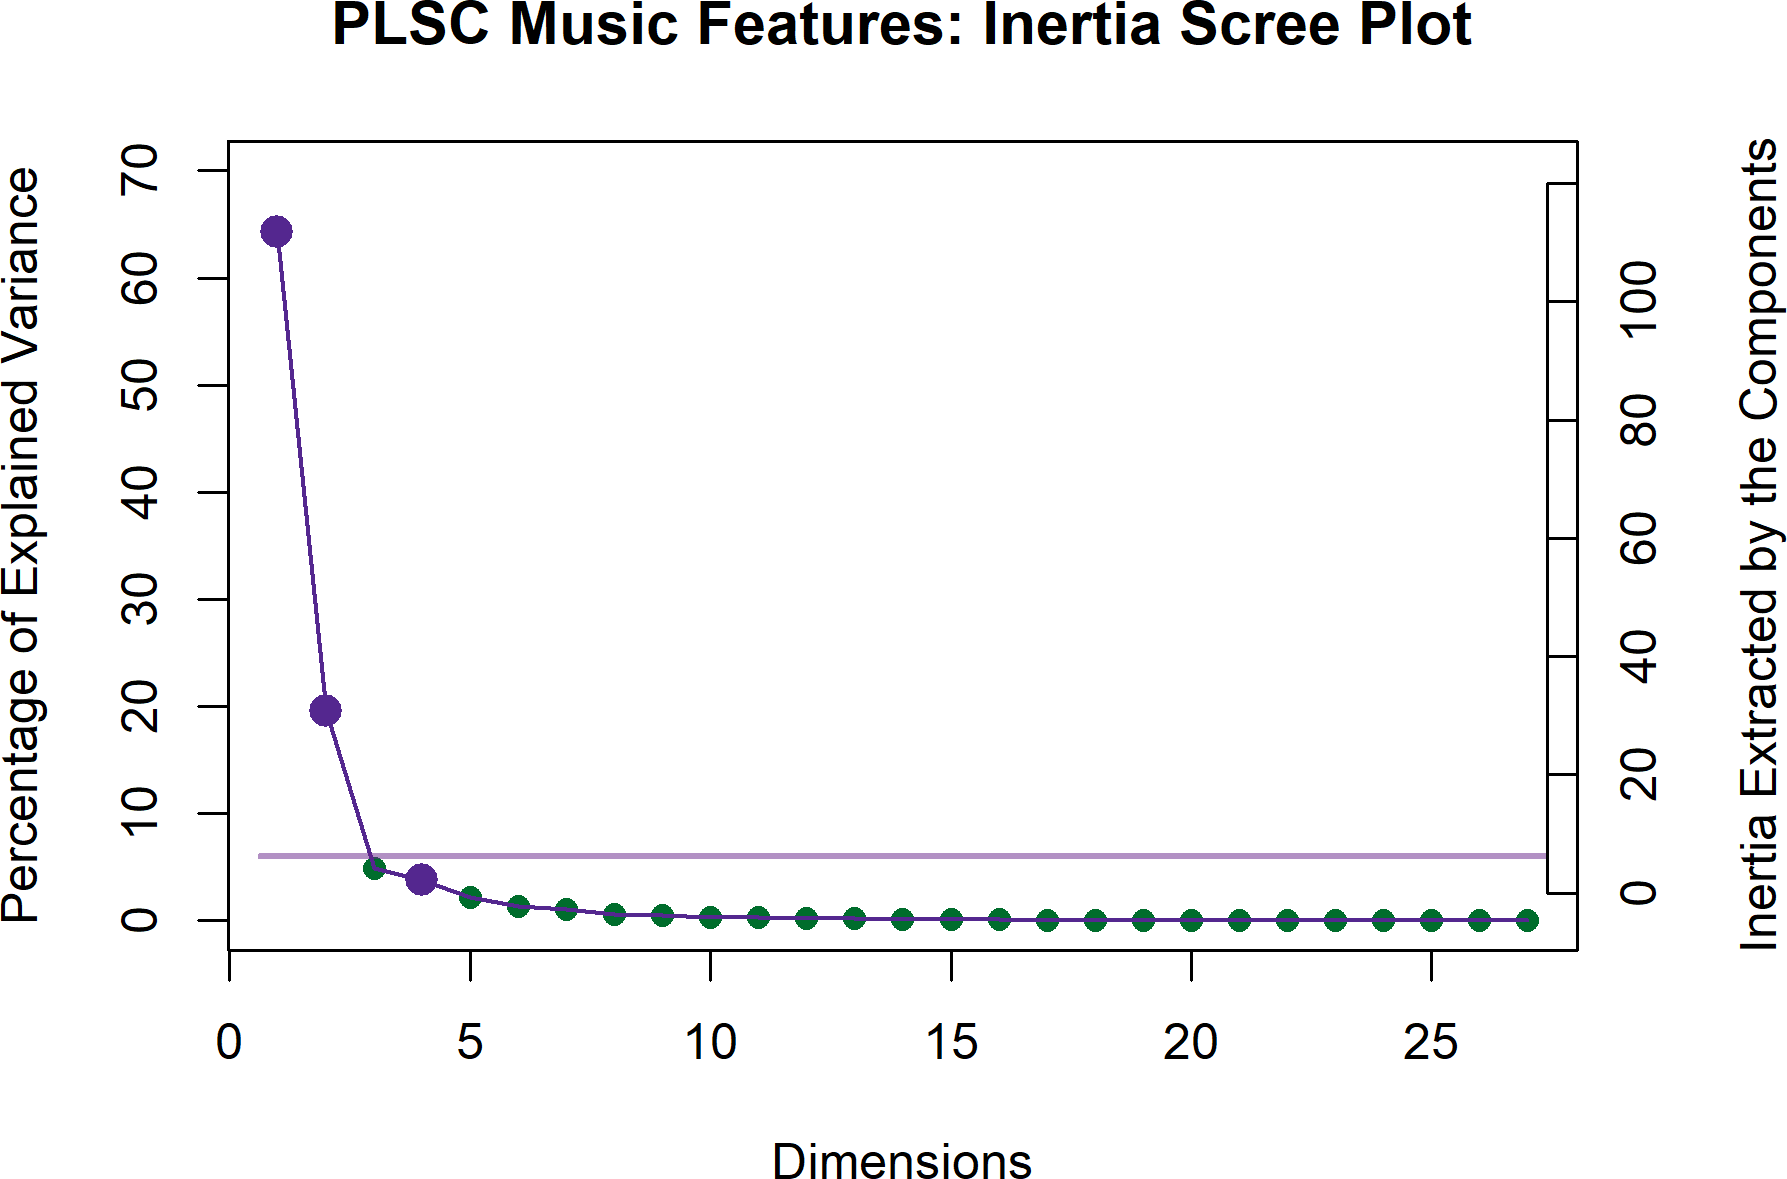
\includegraphics{./Music-Descriptor-Space_files/figure-latex/screePLSC-1.png}
  \caption{ }\label{fig:screePLSC}  
 \end{center}
\end{wrapfigure}

This analysis revealed two dimensions that extracted the majority of the variance (83.79\%), with the first dimension extracted 64.24\% and the second 19.55\%. The scree plot in Figure @fig:screePLSC indicates there are two elbows in this graph, at the 3rd and 5th dimensions, suggesting that further analysis is possible.

The plot below shows which variables from each data table load the most on the first and second dimensions. For the purposes of this visualization, only the variables for which 70\% or more of the variance is explained are shown. The nature of the PLSC also suggests that these are the variables that are most associated with one another between the two tables. The strongest signal on the first dimension juxtaposes the slow and legato musical qualities in the positive direction with the fast, staccato, marcato, and conjunct musical qualities in the negative direction. The adjectives associated with the qualities in the positive direction are ``Dark,'' ``Dull,'' ``Long,'' ``Melancholy,'' ``Sad,'' ``Slow,'' ``Solemn,'' and ``Weak.'' The adjectives associated with the negative direction are ``Bright,'' ``Colorful,'' ``Dancing,'' ``Fast,'' ``Happy,'' and ``Light.''\\
The second dimension identified in the positive direction major harmony and medium dynamics, associated with ``Light,'' ``Round,'' ``Soft,'' and ``Warm.'' The negative direction is driven by the impressionist genre being associated with ``Aggressive,'' ``Complex,'' ``Dense,'' ``Disturbing,'' ``Powerful,'' and ``Surprising.''

\begin{figure}

{\centering 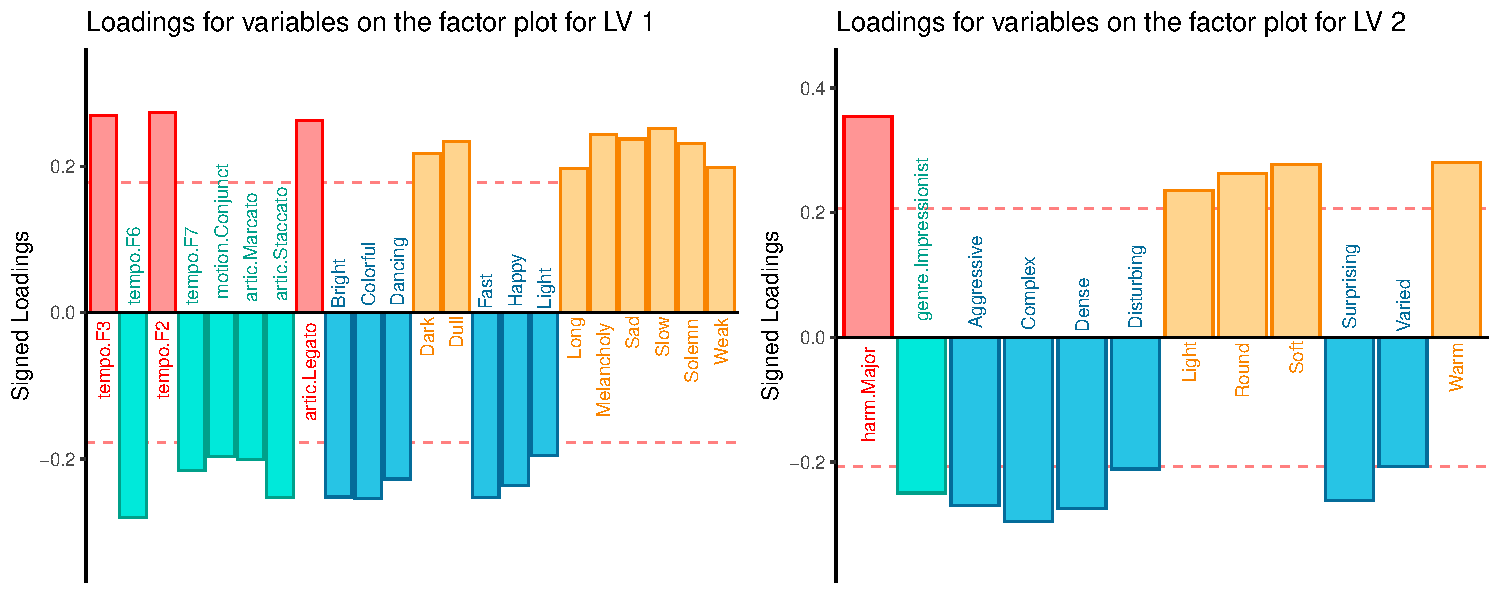
\includegraphics{Music-Descriptor-Space_files/figure-latex/loadingsplsc-1} 

}

\caption{ }\label{fig:loadingsplsc}
\end{figure}

Figures \ref{fig:contsplsc} and \ref{fig:loadingsplsc} show us that there are more variables that contribute significantly to these dimensions than for which a significant portion of the variance is explained. There are similar groups, however: on the first dimension, the tempo variables are contributing significantly, along with some from harmony, density, genre, dynamics, motion, range, and articulation. The adjectives contributing significantly are Bright, colorful, Dancing, Fast, Happy, Light, and Valiant in the positive direction, and Dark, Dull, Long, Melancholy, Monotonous, Sad, Slow, Solemn, and Weak in the negative direction. This juxtaposes some negatively and positively valenced adjectives, and identifies which musical qualities contribute to the valence dimension. Even though some of these variables did not contribute significantly in their plots above (see Figures \ref{fig:factormapsA} and \ref{fig:factormapsQ}), their appearance here indicates that they are part of the shared signal between the tables.
One-third of the musical qualities contributing to the second dimension are harmony and genre. Also contributing are the dynamics and contour groups, while contour, articulation, motion, and range show only one or two variables. The adjectives contributing negatively are Aggressive, Complex, Dense, Disturbing, Incisive, Mysterious, Powerful, Surprising, and Varied, and those contributing positively are Light, Round, Soft, Transparent, and Warm.

\begin{figure}

{\centering 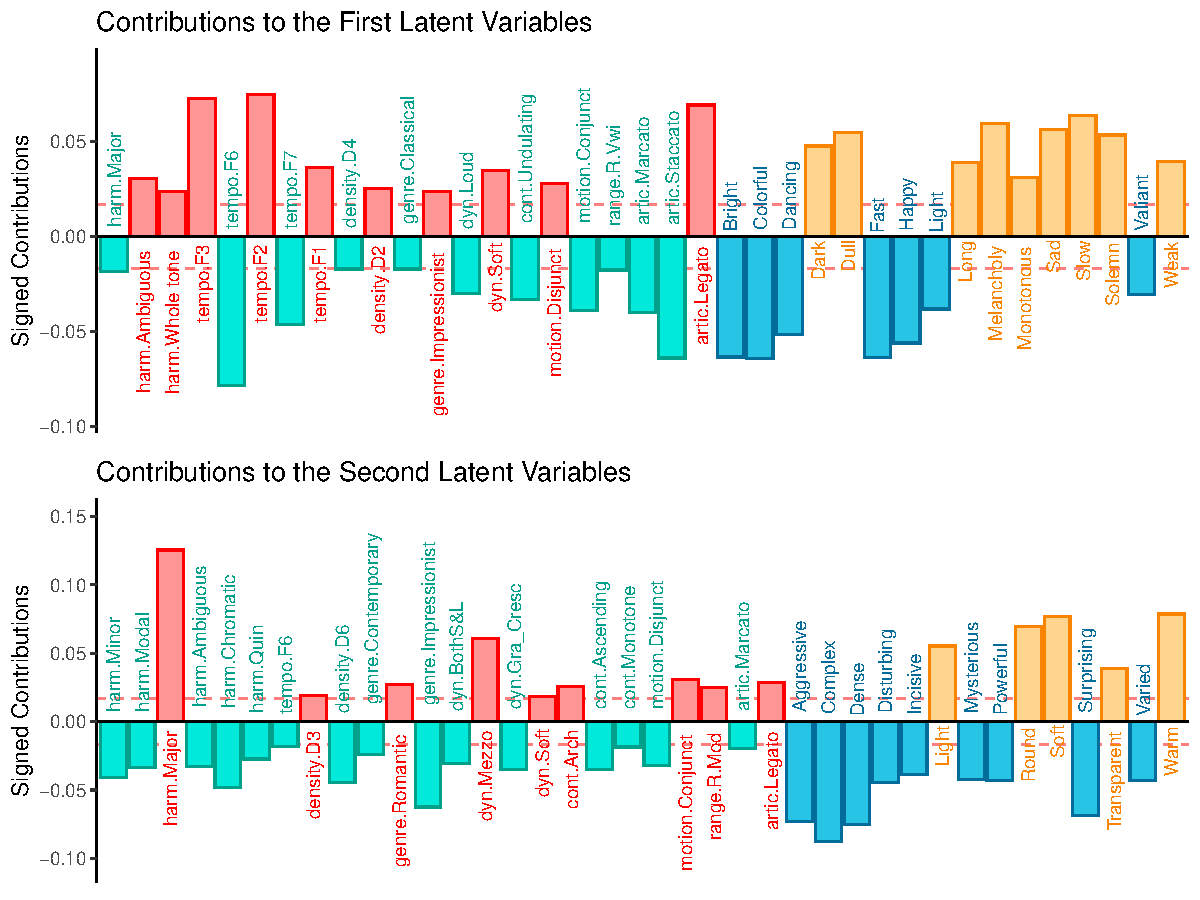
\includegraphics{Music-Descriptor-Space_files/figure-latex/contsplsc-1} 

}

\caption{ }\label{fig:contsplsc}
\end{figure}

\hypertarget{discussion-2}{%
\subsubsection{Discussion}\label{discussion-2}}

The factor score plots for this analysis shows that the first two sets of latent variables extracted by the analysis effectively separate the groups of excerpts into the clusters defined in the HCA for the adjectives survey. The strongest correlated signal between the two data tables separates Excerpts groups 2 and 3 and the second latent variable separates groups 1 and 4. Although there are no factor plots for the variables in this analysis, the valence-arousal plane created by the first two dimensions is still apparent.
This suggests that the excerpts that are more distant from the origin in the first LV plot are defined more by valence than arousal, and those clustered further from the origin on the second LV plot are defined more by arousal than valence. For example, Excerpt 26 is one of the most extreme examples of positive valence, but is much closer to the origin in the second LV plot similarly with Excerpt 27, but with negative valence. This is contrasted with Excerpt 7, which is one of the most negatively valenced stimuli, but also scores very high on arousal, although the confidence interval for that group circles the origin of that plot.

\begin{figure}

{\centering 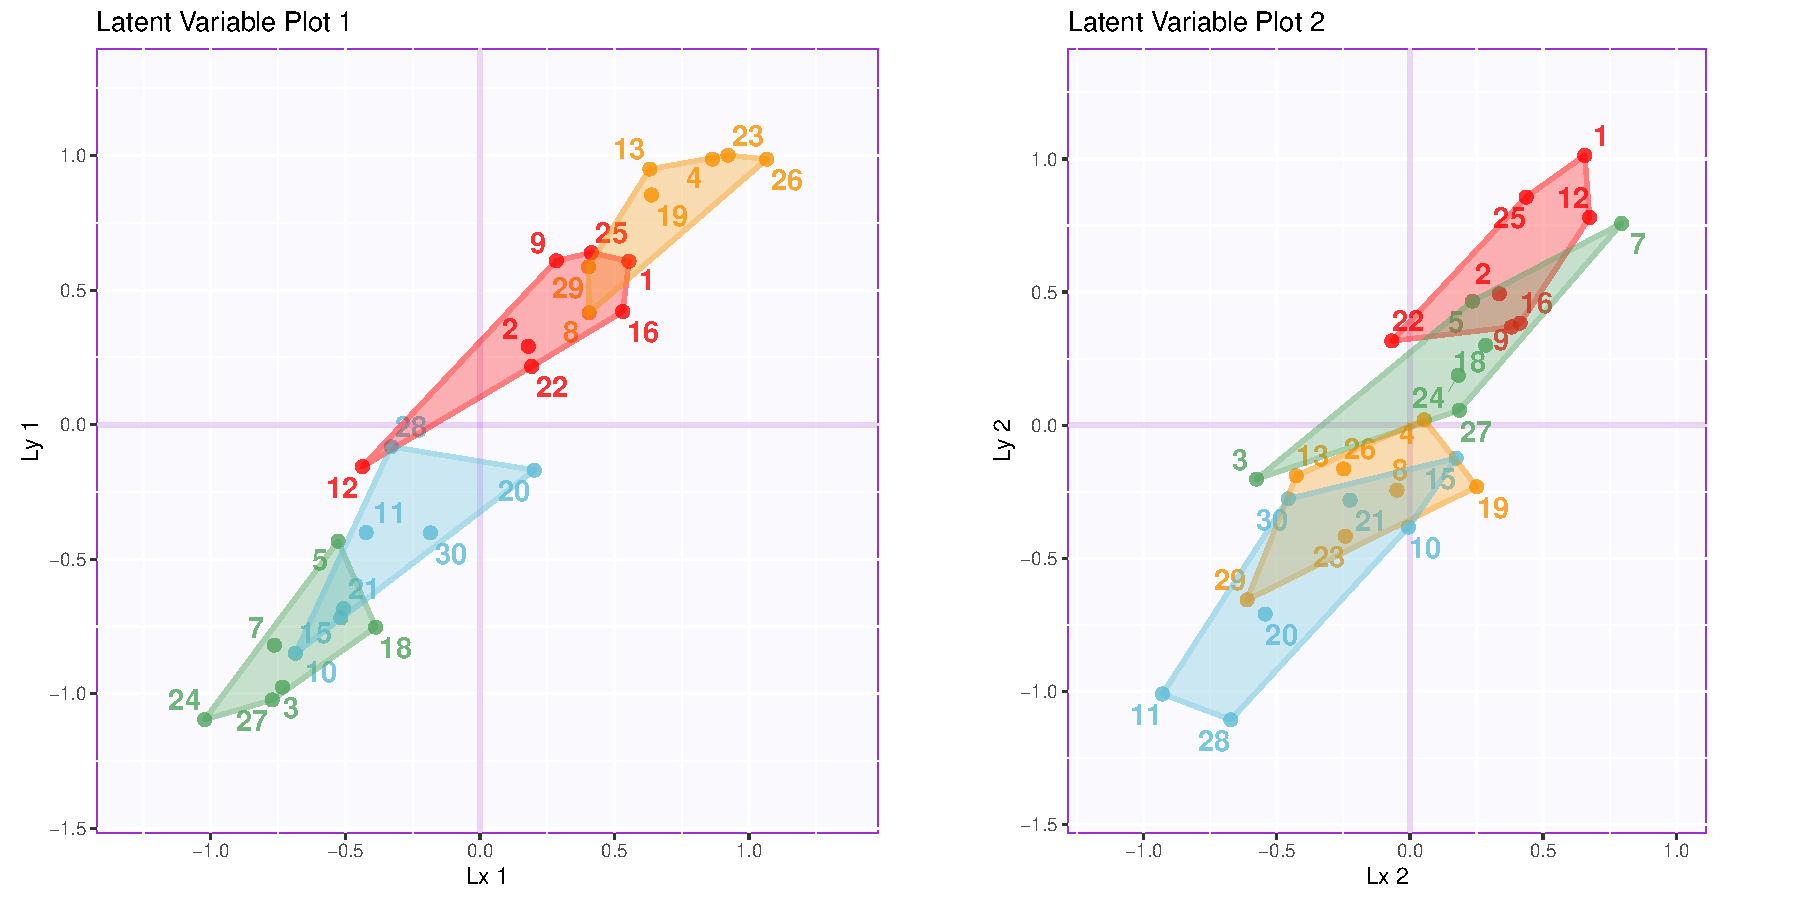
\includegraphics{Music-Descriptor-Space_files/figure-latex/factorplotsPLSC-1} 

}

\caption{ }\label{fig:factorplotsPLSC}
\end{figure}

\hypertarget{general-discussion}{%
\section{General Discussion}\label{general-discussion}}

We used multivariate analyses to explore the musical and cognitive spaces created by participants from France and the United States when responding to a set of new string quartets. These results revealed a clear valence-arousal plane that was common to participants from both countries, but significant differences in the behavior of French and American participants when responding to the stimuli using adjectives, and a space largely defined by genre when evaluating the stimuli using musical qualities. The combined musical and cognitive spaces identified which musical qualities were associated with which descriptors in terms of valence and arousal. Both of these studies involved capturing responses to many stimuli and
One effect observed in Experiment 1 which was not observed in Experiment 2, in which two individual excerpts --- numbers 6 and 14 --- dominate the factor space, requires more explanation. This effect is due to the nature of CA, which is to find the average observation. In a CA, information that is common falls towards the origin --- the center of mass --- of the factor plot, while information that is further from the average, or more rare, ends up further away (Abdi \& Williams, 2010). Therefore, if any individual item on a survey is rated significantly different from the rest of the items, that item can dominate the factor space. In this case we have two such examples: Excerpt 6 was written as a Steve-Reich-esque minimalist, ostinato based excerpt, and excerpt 14 was written to be jazzy. This effect does not appear in Experiment 2 because the AS was designed to evaluate the excerpts more generally on holistic qualities, not to separate the excerpts along specific musical dimensions. Excerpt 6 still appears near the edge of the mental space in Experiment 2, indicating that it is somewhat of an outlier, but does not dominate the space the way it does in the results Experiment 1.
In order to interpret the space without the effects of Excerpts 6 and 14, those two excerpts were removed from the dataset for the initial analysis and then included as \emph{supplementary projections}, sometimes also referred to as \emph{out of sample observations}. This allowed us to evaluate what information is shared by the outliers and the other elements in the dataset without having the outliers dominate the visualization of the factor space. The fact that this was a necessary step supports our interpretation that the factor space is defined by genre. The supplementary projections' location in the factor space shows that there is some shared information between genres. If the supplementary observations had projected onto the origin or very close to it, that would indicate that they shared no information with the other variables.
One takeaway from these results is that a deep understanding of the stimuli may help to predict the approximate dimensionality of the solution factor space, and when designing surveys or stimuli, multiple items per group, or presumed dimension, are needed. The outliers distorting the factor space that were observed in the present study are analogous to the single noisy dimension described in the introduction. The noise contributed by Excerpt 6 is also present in the results of Experiment 2, possibly because untrained participants are less likely to be familiar with minimalism than the trained participants in Experiment 1, but the results are robust to that noise because the participants were not asked to rate the excerpts on any explicit dimensions or qualities.\\
The significant results for the participants in Experiment 2 that were not observed in Experiment 1 suggest that this experimental paradigm works as intended. Significant differences between the experts' ratings of the stimuli would have indicated that the experts were inconsistent and thus not reliable raters of the music. The significant differences between the French and American adjectives surveys indicate that language connotations do have a significant impact on how participants rate the stimuli. MFA revealed what those differences were and highlighted further possibilities for analysis.

\hypertarget{limitations-future-directions}{%
\subsection{Limitations \& future directions}\label{limitations-future-directions}}

Although we evaluate the scores and ratings of participants from different countries, we recognize that the issue of multiculturality is not addressed to a significant degree in this study, because France and the United States are both western countries that share Western musical culture. To truly address this question, an experiment would need to include participants from multiple, contrasting musical cultures, with languages that are more distant than English and French. However, specific musical qualities, like harmony, may not apply or translate well to other musical cultures, because the concepts of melodic and harmonic material are not the same across all musical cultures (Cohn et al., 2001; Raman \& Dowling, 2017). Therefore the specific questions included in the QS would need to be adjusted.\\
Although we suggest that data collected in this way have a much greater hypothetical reach, we recognize that the data collected for these experiments represent a convenience sample, and many of the participants were students. However, these limitations could be easily remedied in future studies.
Another question that fell beyond the scope of this study what the source of the semantic drift between languages is. Although illustrated in Figure \ref{fig:mfasbs}, the source of the differences between French and American participants is not entirely clear. These differences may not come from cultural aspects of music listening, but linguistic sources, including the adjectives' frequency of use in either language or the cultural associations with the words (B. Thompson et al., 2020), or even the physical characteristics of the words themselves (Reilly et al., 2012). Diving more into those questions would be a fascinating future study. Another interesting study would be to use adjectives from specific domains, to see how music maps onto different sensory spaces, for example textural words, like `moist,' `slimy,' `dry,' `puckered,' `smooth.'\\
Finally, the results of this study and possible extensions, in conjunction with studies that have already evaluated music perception non-verbally, may provide insight into the way in which people without language react to music, such as nonverbal autistic people.

\hypertarget{conclusions}{%
\section{Conclusions}\label{conclusions}}

Expanding the collection and analytical paradigms, and thus expanding scientific scope and perspective, has the added benefit of increasing reach. By expanding the ways in which we collect data, including developing investigative paradigms that are accessible on mobile platforms and that reduce participant demand while maintaining rigor and integrity, we are able to more readily and consistently reach a broader participant population, that might normally be excluded from everday research paradigms, specifically racially and ethnically diverse populations, poorer populations, those with limited access to transportation, or who have a disability, or are immunocompromised. Pairing this kind of data gathering with appropriate analysis will help maintain scientific integrity. The number of ways that exist to analyze data from a single set of experiments is considerable, and the results of each analysis illuminate different parts of the story behind the data. Not every form of analysis is appropriate in every context, but understanding how, and perhaps more importantly when, to apply an analytical technique is vital to uncovering new perspectives or insights.

\newpage

\hypertarget{references}{%
\section{References}\label{references}}

\begingroup
\setlength{\parindent}{-0.5in}
\setlength{\leftskip}{0.5in}

\hypertarget{refs}{}
\begin{CSLReferences}{1}{0}
\leavevmode\hypertarget{ref-Abdi2010d}{}%
Abdi, H., \& Williams, L. J. (2010). {Correspondence Analysis}. In N. Salkind (Ed.), \emph{Encyclopedia of research design}. Sage.

\leavevmode\hypertarget{ref-Abdi2013a}{}%
Abdi, H., \& Williams, L. J. (2013). {Partial Least Squares Methods: Partial Least Squares Correlation and Partial Least Square Regression}. In B. Reisfeld \& A. N. Mayeno (Eds.), \emph{Methods in molecular biology: Computational toxicology volume II} (Vol. 930, pp. 549--579). Springer Science+Business Media, LLC. \url{https://doi.org/10.1007/978-1-62703-059-5}

\leavevmode\hypertarget{ref-Abdi2013}{}%
Abdi, H., Williams, L. J., \& Valentin, D. (2013). {Multiple factor analysis: Principal component analysis for multitable and multiblock data sets}. \emph{Wiley Interdisciplinary Reviews: Computational Statistics}, \emph{5}, 149--179. \url{https://doi.org/10.1002/wics.1246}

\leavevmode\hypertarget{ref-Ares2010}{}%
Ares, G., Deliza, R., Barreiro, C., Giménez, A., \& Gámbaro, A. (2010). {Comparison of two sensory profiling techniques based on consumer perception}. \emph{Food Quality and Preference}, \emph{21}(4), 417--426. \url{https://doi.org/10.1016/j.foodqual.2009.10.006}

\leavevmode\hypertarget{ref-Balkwill2004}{}%
Balkwill, L. L., Thompson, W. F., \& Matsunaga, R. (2004). {Recognition of emotion in Japanese, Western, and Hindustani music by Japanese listeners}. \emph{Japanese Psychological Research}, \emph{46}(4), 337--349. \url{https://doi.org/10.1111/j.1468-5584.2004.00265.x}

\leavevmode\hypertarget{ref-Balkwill1999}{}%
Balkwill, L., \& Thompson, W. F. (1999). {A Cross-Cultural Investigation of the Perception of Emotion in Music : Psychophysical and Cultural Cues}. \emph{Music Perception: An Interdisciplinary Journal}, \emph{17}(1), 43--64. \url{https://doi.org/10.2307/40285811}

\leavevmode\hypertarget{ref-Bartlett1980}{}%
Bartlett, J. C., \& Dowling, W. J. (1980). {Recognition of transposed melodies: A key-distance effect in developmental perspective}. \emph{Journal of Experimental Psychology: Human Perception and Performance}, \emph{6}(3), 501--515. \url{https://doi.org/10.1037/0096-1523.6.3.501}

\leavevmode\hypertarget{ref-Battcock2019}{}%
Battcock, A., \& Schutz, M. (2019). {Acoustically expressing affect}. \emph{Music Perception}, \emph{37}(1), 66--91. \url{https://doi.org/10.1525/MP.2019.37.1.66}

\leavevmode\hypertarget{ref-Benzecri1973}{}%
Benzécri, J.-P. (1973). \emph{{L'analyse des données.}} Dunod.

\leavevmode\hypertarget{ref-Berry2011}{}%
Berry, K. J., Johnston, J. E., \& Mielke, P. W. (2011). {Permutation methods}. \emph{Wiley Interdisciplinary Reviews: Computational Statistics}, \emph{3}(6), 527--542. \url{https://doi.org/10.1002/wics.177}

\leavevmode\hypertarget{ref-Bigand2006}{}%
Bigand, E., \& Poulin-Charronnat, B. (2006). {Are we "experienced listeners"? A review of the musical capacities that do not depend on formal musical training}. \emph{Cognition}, \emph{100}(1), 100--130. \url{https://doi.org/10.1016/j.cognition.2005.11.007}

\leavevmode\hypertarget{ref-Bigand2005}{}%
Bigand, E., Vieillard, S., Madurell, F., Marozeau, J., \& Dacquet, A. (2005). {Multidimensional scaling of emotional responses to music: The effect of musical expertise and of the duration of the excerpts}. \emph{Cognition and Emotion}, \emph{19}(8), 1113--1139. \url{https://doi.org/10.1080/02699930500204250}

\leavevmode\hypertarget{ref-Borg2005}{}%
Borg, I., \& Groenen, P. J. F. (2005). \emph{{Modern Multidimensional Scaling}} (2nd ed., Vol. 36). Springer Science+Business Media, Inc.

\leavevmode\hypertarget{ref-BrunerII1990}{}%
Bruner II, G. C. (1990). {Music, Mood, and Marketing}. \emph{Journal of Marketing}, \emph{October}, 94--104.

\leavevmode\hypertarget{ref-Cohn2001}{}%
Cohn, R., Hyer, B., Dahlhaus, C., Anderson, J., \& Wilson, C. (2001). \emph{{Harmony}}. Oxford University Press.

\leavevmode\hypertarget{ref-Coombs1956}{}%
Coombs, C. H., Milholland, J. E., \& Womer, F. B. (1956). {The assessment of partial knowledge}. \emph{Educational and Psychological Measurement}, \emph{16}(1), 13--37. \url{https://doi.org/10.1177/001316445601600102}

\leavevmode\hypertarget{ref-Cowen2020}{}%
Cowen, A. S., Fang, X., Sauter, D., \& Keltner, D. (2020). {What music makes us feel: At least 13 dimensions organize subjective experiences associated with music across different cultures}. \emph{Proceedings of the National Academy of Sciences of the United States of America}, \emph{117}(4), 1924--1934. \url{https://doi.org/10.1073/pnas.1910704117}

\leavevmode\hypertarget{ref-Darrow1987}{}%
Darrow, A. A., Haack, P., \& Kuribayashi, F. (1987). {Descriptors and Preferences for Eastern and Western Musics by Japanese and American Nonmusic Majors}. \emph{Journal of Research in Music Education}, \emph{35}(4), 237--248. \url{https://doi.org/10.2307/3345076}

\leavevmode\hypertarget{ref-Dowling1978a}{}%
Dowling, W. J. (1978). {Scale and Contour: Two Components of a Theory of Memory for Melodies}. \emph{Psychological Review}, \emph{85}(4), 341--354. \url{https://doi.org/10.1037/0033-295X.85.4.341}

\leavevmode\hypertarget{ref-Escofier-Cordier1965}{}%
Escofier-Cordier, B. (1965). \emph{{L'analyse des correspondances}} {[}Doctoral Thesis{]}. Universit{é} de Rennes.

\leavevmode\hypertarget{ref-Fritz2009}{}%
Fritz, T., Jentschke, S., Gosselin, N., Sammler, D., Peretz, I., Turner, R., Friederici, A. D., \& Koelsch, S. (2009). {Universal Recognition of Three Basic Emotions in Music}. \emph{Current Biology}, \emph{19}(7), 573--576. \url{https://doi.org/10.1016/j.cub.2009.02.058}

\leavevmode\hypertarget{ref-Gray1967}{}%
Gray, P. H., \& Wheeler, G. E. (1967). {The Semantic Differential as an Instrument to Examine the Recent Folksong Movement}. \emph{Journal of Social Psychology}, \emph{72}(2), 241--247. \url{https://doi.org/10.1080/00224545.1967.9922321}

\leavevmode\hypertarget{ref-Greenacre1984}{}%
Greenacre, M. J. (1984). \emph{{Theory and Applications of Correspondence Analysis}}. Academic Press.

\leavevmode\hypertarget{ref-Gregory1996}{}%
Gregory, A. H., \& Varney, N. (1996). {Cross-cultural comparisons in the affective response to music}. \emph{Psychology of Music}, \emph{24}(1), 47--52. \url{https://doi.org/10.1177/0305735696241005}

\leavevmode\hypertarget{ref-Hesterberg2011}{}%
Hesterberg, T. (2011). {Bootstrap}. \emph{Wiley Interdisciplinary Reviews: Computational Statistics}, \emph{3}(6), 497--526. \url{https://doi.org/10.1002/wics.182}

\leavevmode\hypertarget{ref-Juslin2010}{}%
Juslin, P. N., \& Sloboda, J. A. (Eds.). (2010). \emph{{Handbook of music and emotion: Theory, research, applications.}} Oxford University Press.

\leavevmode\hypertarget{ref-Juslin2008a}{}%
Juslin, P. N., \& Västfjäll, D. (2008). {All emotions are not created equal: Reaching beyond the traditional disputes}. \emph{Behavioral and Brain Sciences}, \emph{31}, 559--621. \url{https://doi.org/doi:10.1017/S0140525X08005554\%20Patrik}

\leavevmode\hypertarget{ref-Katz1933}{}%
Katz, D., \& Braly, K. (1933). {Racial stereotypes of one hundred college students}. \emph{Journal of Abnormal and Social Psychology}, \emph{28}(3), 280--290. \url{https://doi.org/10.1037/h0074049}

\leavevmode\hypertarget{ref-Kennedy2013}{}%
Kennedy, J., Kennedy, M., \& Rutherford-Johnson, T. (2013). \emph{Harmony} (6th ed.). Oxford University Press.

\leavevmode\hypertarget{ref-Kopacz2005}{}%
Kopacz, M. (2005). {Personality and music preferences: The influence of personality traits on preferences regarding musical elements}. \emph{Journal of Music Therapy}, \emph{42}(3), 216--239. \url{https://doi.org/10.1093/jmt/42.3.216}

\leavevmode\hypertarget{ref-Krishnan2011}{}%
Krishnan, A., Williams, L. J., McIntosh, A. R., \& Abdi, H. (2011). {Partial Least Squares (PLS) methods for neuroimaging: A tutorial and review}. \emph{NeuroImage}, \emph{56}(2), 455--475. \url{https://doi.org/10.1016/j.neuroimage.2010.07.034}

\leavevmode\hypertarget{ref-Ladinig2012}{}%
Ladinig, O., \& Glenn Schellenberg, E. (2012). {Liking unfamiliar music: Effects of felt emotion and individual differences}. \emph{Psychology of Aesthetics, Creativity, and the Arts}, \emph{6}(2), 146--154. \url{https://doi.org/10.1037/a0024671}

\leavevmode\hypertarget{ref-Madsen1997}{}%
Madsen, C. K. (1997). {Emotional Response to Music as Measured by the Two-Dimensional CRDI}. \emph{Journal of Music Therapy}, \emph{34}(3), 187--199. \url{https://doi.org/10.1093/jmt/34.3.187}

\leavevmode\hypertarget{ref-Meyners2014}{}%
Meyners, M., \& Castura, J. (2014). {Check-All-That-Apply Questions}. In \emph{Novel techniques in sensory characterization and consumer profiling} (pp. 271--306). CRC Press/Taylor {\&} Francis. \url{https://doi.org/10.1201/b16853-12}

\leavevmode\hypertarget{ref-Osgood1955}{}%
Osgood, C. E., \& Suci, G. J. (1955). {Factor analysis of meaning}. \emph{Journal of Experimental Psychology}, \emph{50}(5), 325--338. \url{https://doi.org/10.1037/h0043965}

\leavevmode\hypertarget{ref-Raman2016}{}%
Raman, R., \& Dowling, W. J. (2016). {Real-Time Probing of Modulations in South Indian Classical (Carnātic) Music by Indian and Western Musicians}. \emph{Music Perception}, \emph{33}(3), 367--393. \url{https://doi.org/10.1525/MP.2016.33.03.367}

\leavevmode\hypertarget{ref-Raman2017}{}%
Raman, R., \& Dowling, W. J. (2017). {Perception of modulations in south indian classical (carnatic) music by student and teacher musicians: A cross-cultural study}. \emph{Music Perception}, \emph{34}(4), 424--437.

\leavevmode\hypertarget{ref-Reilly2012}{}%
Reilly, J., Westbury, C., Kean, J., \& Peelle, J. E. (2012). {Arbitrary symbolism in natural language revisited: When word forms carry meaning}. \emph{PLoS ONE}, \emph{7}(8). \url{https://doi.org/10.1371/journal.pone.0042286}

\leavevmode\hypertarget{ref-Roda2014}{}%
Rodà, A., Canazza, S., \& De Poli, G. (2014). {Clustering affective qualities of classical music: Beyond the valence-arousal plane}. \emph{IEEE Transactions on Affective Computing}, \emph{5}(4), 364--376. \url{https://doi.org/10.1109/TAFFC.2014.2343222}

\leavevmode\hypertarget{ref-Thompson2020}{}%
Thompson, B., Roberts, S. G., \& Lupyan, G. (2020). {Cultural influences on word meanings revealed through large-scale semantic alignment}. \emph{Nature Human Behaviour}, \emph{4}(10), 1029--1038. \url{https://doi.org/10.1038/s41562-020-0924-8}

\leavevmode\hypertarget{ref-Thompson1994}{}%
Thompson, W. F. (1994). {Sensitivity to combinations of musical parameters: Pitch with duration, and pitch pattern with durational pattern}. \emph{Perception {\&} Psychophysics}, \emph{56}(3), 363--374. \url{https://doi.org/10.3758/BF03209770}

\leavevmode\hypertarget{ref-Tucker1958}{}%
Tucker, L. R. (1958). {An inter-battery method of factor analysis}. \emph{Psychometrika}, \emph{23}(2), 111--136. \url{https://doi.org/10.1007/BF02289009}

\leavevmode\hypertarget{ref-Valentin2012}{}%
Valentin, D., Chollet, S., Lelièvre, M., \& Abdi, H. (2012). {Quick and dirty but still pretty good: a review of new descriptive methods in food science}. \emph{International Journal of Food Science {\&} Technology}, 1--16. \url{https://doi.org/10.1111/j.1365-2621.2012.03022.x}

\leavevmode\hypertarget{ref-Wallmark2019}{}%
Wallmark, Z. (2019). {A corpus analysis of timbre semantics in orchestration treatises}. \emph{Psychology of Music}, \emph{47}(4), 585--605. \url{https://doi.org/10.1177/0305735618768102}

\leavevmode\hypertarget{ref-Wedin1969}{}%
Wedin, L. (1969). {Dimension Analysis of Emotional Expression in Music}. \emph{Swedish Journal of Musicology}, \emph{51}, 119--140.

\leavevmode\hypertarget{ref-Wedin1972}{}%
Wedin, L. (1972). {Evaluation of a Three-Dimensional Model of Emotional Expression in Music}. \emph{The Psychological Laboratories}, \emph{54}(349), 1--17.

\leavevmode\hypertarget{ref-Zacharakis2014}{}%
Zacharakis, A., Pastiadis, K., \& Reiss, J. D. (2014). {An Interlanguage Study of Musical Timbre Semantic Dimensions and Their Acoustic Correlates}. \emph{Music Perception: An Interdisciplinary Journal}, \emph{31}(4), 339--358. \url{https://doi.org/10.1525/MP.2014.31.4.339}

\leavevmode\hypertarget{ref-Zacharakis2015}{}%
Zacharakis, A., Pastiadis, K., \& Reiss, J. D. (2015). {An Interlanguage Unification of Musical Timbre: Bridging Semantic, Perceptual, and Acoustic Dimensions}. \emph{Music Perception: An Interdisciplinary Journal}, \emph{32}(4), 394--412. \url{https://doi.org/10.1525/MP.2015.32.4.394}

\end{CSLReferences}

\endgroup


\end{document}
